
\documentclass[11pt]{article}

\usepackage{deauthor}
\usepackage{times}
\usepackage{authblk}
\usepackage{graphicx}

\usepackage{float,color}
\usepackage{makecell}
\usepackage{comment}
%\usepackage[normalem]{ulem}
\usepackage{algorithmic}
\usepackage{algorithm}
\usepackage{array}
\usepackage{xurl}
\usepackage{subfig}
\usepackage{caption}
\usepackage{enumitem,kantlipsum}
\usepackage{placeins}
\usepackage{amsmath}
\usepackage{diagbox}
\usepackage{chngpage}
\usepackage{subfig}


\newcommand{\gchecker}{\textsc{KompaRe}}
\newtheorem{pro-stat}{Problem Definition}
\newcommand{\hide}[1]{}
\newcommand{\hh}[1]{{\small\color{red}{\bf hh: #1}}}
\newcommand{\lliu}[1]{{\small\color{blue}{\bf lihui: #1}}}
\newcommand{\heng}[1]{{\small\color{red}{\bf heng: #1}}}
\newcommand{\bx}[1]{{\small\color{green}{\bf Boxin: #1}}}
\newcommand{\mkclean}{
	\renewcommand{\hh}[1]{}
	\renewcommand{\bx}[1]{}
	\renewcommand{\heng}[1]{}
	\renewcommand{\lliu}[1]{}
}



\mkclean
\begin{document}


\title{Knowledge Graph Comparative Reasoning for Fact Checking: Problem Definition and Algorithms}



% \author{Junchao Chen,\quad Suyash Gupta$^{\dagger}$,\quad Sajjad Rahnama,\quad Mohammad Sadoghi\\
%     \textit{Moka Blox LLC} \\
%     Exploratory Systems Lab \\
%     University of California, Davis \\
%     $^{\dagger}$University of California, Berkeley
% }


\author{Lihui Liu*, Ruining Zhao*,  Boxin Du$\ddagger$\footnote{The publication was written prior to the employee joining Amazon.}, Yi Ren Fung*, Heng Ji*, Jiejun Xu$\dagger$, Hanghang Tong* \\
  *Department of Computer Science, University of Illinois at Urbana Champaign \\
  $\dagger$HRL Laboratories, LLC., jxu@hrl.com \\
  $\ddagger$Amazon, boxin@amazon.com\\
  %\institution{$\dagger$jxu@hrl.com}
  *{lihuil2, ruining9, yifung2, hengji, htong}@illinois.edu
}


%


\maketitle

\begin{abstract}


Knowledge graphs are ubiquitous data structure which have been used in many applications. 
Knowledge graph reasoning aims to discover or infer knowledge based on existing information in the knowledge graph.
However, most of the existing works belong to {\em point-wise} approaches, which perform reasoning w.r.t. a single piece of clue.
Comparative reasoning over knowledge graph focuses on inferring commonality and inconsistency with respect to multiple pieces of clues which is a new research direction and can be applied to many applications. 
In this paper, we formally give the definition of comparative reasoning and propose several different methods to tackle comparative reasoning in both pairwise and collective cases. 
The idea of the proposed methods is that we find a knowledge segment from the knowledge graph to best represent the semantic meaning of the given claim, and reasons according to it.
We perform extensive empirical evaluations on real-world datasets to demonstrate that the proposed methods have good performances.




\end{abstract}



\section{Introduction}




Knowledge graphs are ubiquitous data structure which are used to store really world entities (e.g., {\tt Alan Turing}) and their relations ({\tt Alan Turing}, {\tt wasBornIn}, {\tt United Kingdom}).
Since the debut in 2012, several widely used knowledge graphs have been proposed, which include Yago, Wikidata, Freebase and so on.
Knowledge graph reasoning which aims to discover/explain existing knowledge or infer new knowledge from existing information in the knowledge graph has emerged as an important research direction over the last few years ~\cite{binet}.
%It is the mainstay of many applications, such as question answering ~\cite{}, recommender systems ~\cite{}, fact checking ~\cite{} and many more.





Despite the great achievement in both academia and industry,
most of the existing works on knowledge graph reasoning belong to the {\em point-wise} approaches, which perform reasoning w.r.t. {\em a single piece of clue} (e.g., a triple ~\cite{transE}, a multi-hop query ~\cite{binet}, a complex query graph ~\cite{lihui}). For example in fact checking, given {\em a claim} (e.g., represented as a triple of the knowledge graph), it decides whether the claim is authentic or falsified ~\cite{kgminer, KL}.
However, {\em comparative reasoning} (~\cite{kompare, prototype_liu}) is rarely studied.
Different from point-wise reasoning (or reasoning over knowledge graph).
{\em Comparative reasoning} over knowledge graph ~\cite{kompare} focuses on inferring commonality and/or inconsistency with respect to multiple pieces of clues (e.g., multiple claims about a news article), which is a new research direction over knowledge graphs and can be widely applied to other applications, e.g., fact checking.



Comparative reasoning has many unique advantages compared with point-wise (single claim) fact checking.
This is because in many real-world situations, e.g., multimodal fake news detection ~\cite{multimodal}, single claim fact checking alone is insufficient, while
comparative reasoning
offers a more complete picture w.r.t. the input clues,
which in turn helps the users discover the subtle patterns (e.g., inconsistency) that would be invisible by point-wise approaches. When we verify the two claims/triples at the same time, the result may be inconsistent even though each claim/triple itself is consistent if we evaluate it individually.
Figure ~\ref{inconsistency} gives an example to illustrate the power of comparative reasoning.
Suppose there is a multi-modal news article and we wish to verify its truthfulness. To this end, two query graphs are extracted from the given news, respectively. One query graph contains all the information from the text, and the other contains the information from the image. If we perform point-wise reasoning to check each of these two query graphs {\em separately}, both seem to be true. However, if we perform reasoning w.r.t. both query graphs simultaneously, and by {\em comparison}, we could discover the subtle inconsistency between them (i.e., the different air plane types, the difference in maximum flying distances). In addition, comparative reasoning can also be used in knowledge graph expansion, integration and completion ~\cite{kompare}.


In this paper, we address the problem of comparative reasoning.
We mainly focus on two problems: pairwise comparative reasoning and collective comparative reasoning. To be specific, we address two key challenges as follows.
We leverage graph neural network and graph kernel to reveal the commonality and inconsistency among input clues according to the information in the background knowledge graph.
We propose several different algorithms and demonstrate their effectiveness. A common building block of comparative reasoning is {\em knowledge segment}, which is a small connection subgraph of a given clue (e.g., a triple or part of it) to summarize its semantic context.
Based on that, we present core algorithms to enable both {\em pairwise} reasoning and {\em collective} reasoning.
The key idea is to use the structure and semantic information in knowledge segments to help discover vague contradictions.

The main contributions of the paper are
\begin{itemize} %\itemsep -1pt
    \item {\bf Problem Definition.} We introduce comparative reasoning over knowledge graphs, which complements and expands
    the existing point-wise reasoning capabilities.
    \item {\bf Algorithms.} We propose a family of comparative reasoning algorithms which can solve both pairwise comparative reasoning and collective comparative reasoning.
    \item {\bf Empirical Evaluations.} We perform extensive empirical evaluations to demonstrate the efficacy of our proposed methods.
\end{itemize}


The rest of the paper is organized as follows. Section ~\ref{problem_definition} introduces notations used in this paper and gives the problem definition.
Section ~\ref{ks_extractt} introduces how to extract the knowledge segment from the knowledge graph.
Section ~\ref{methods} proposes different methods to solve comparative reasoning problem.
The experiment results are presented in Section ~\ref{experiments}, and the related work is reviewed in Section ~\ref{related-work}. Finally, the paper is concluded in Section ~\ref{conclusion}.

\begin{figure*}[ht!]
\centering
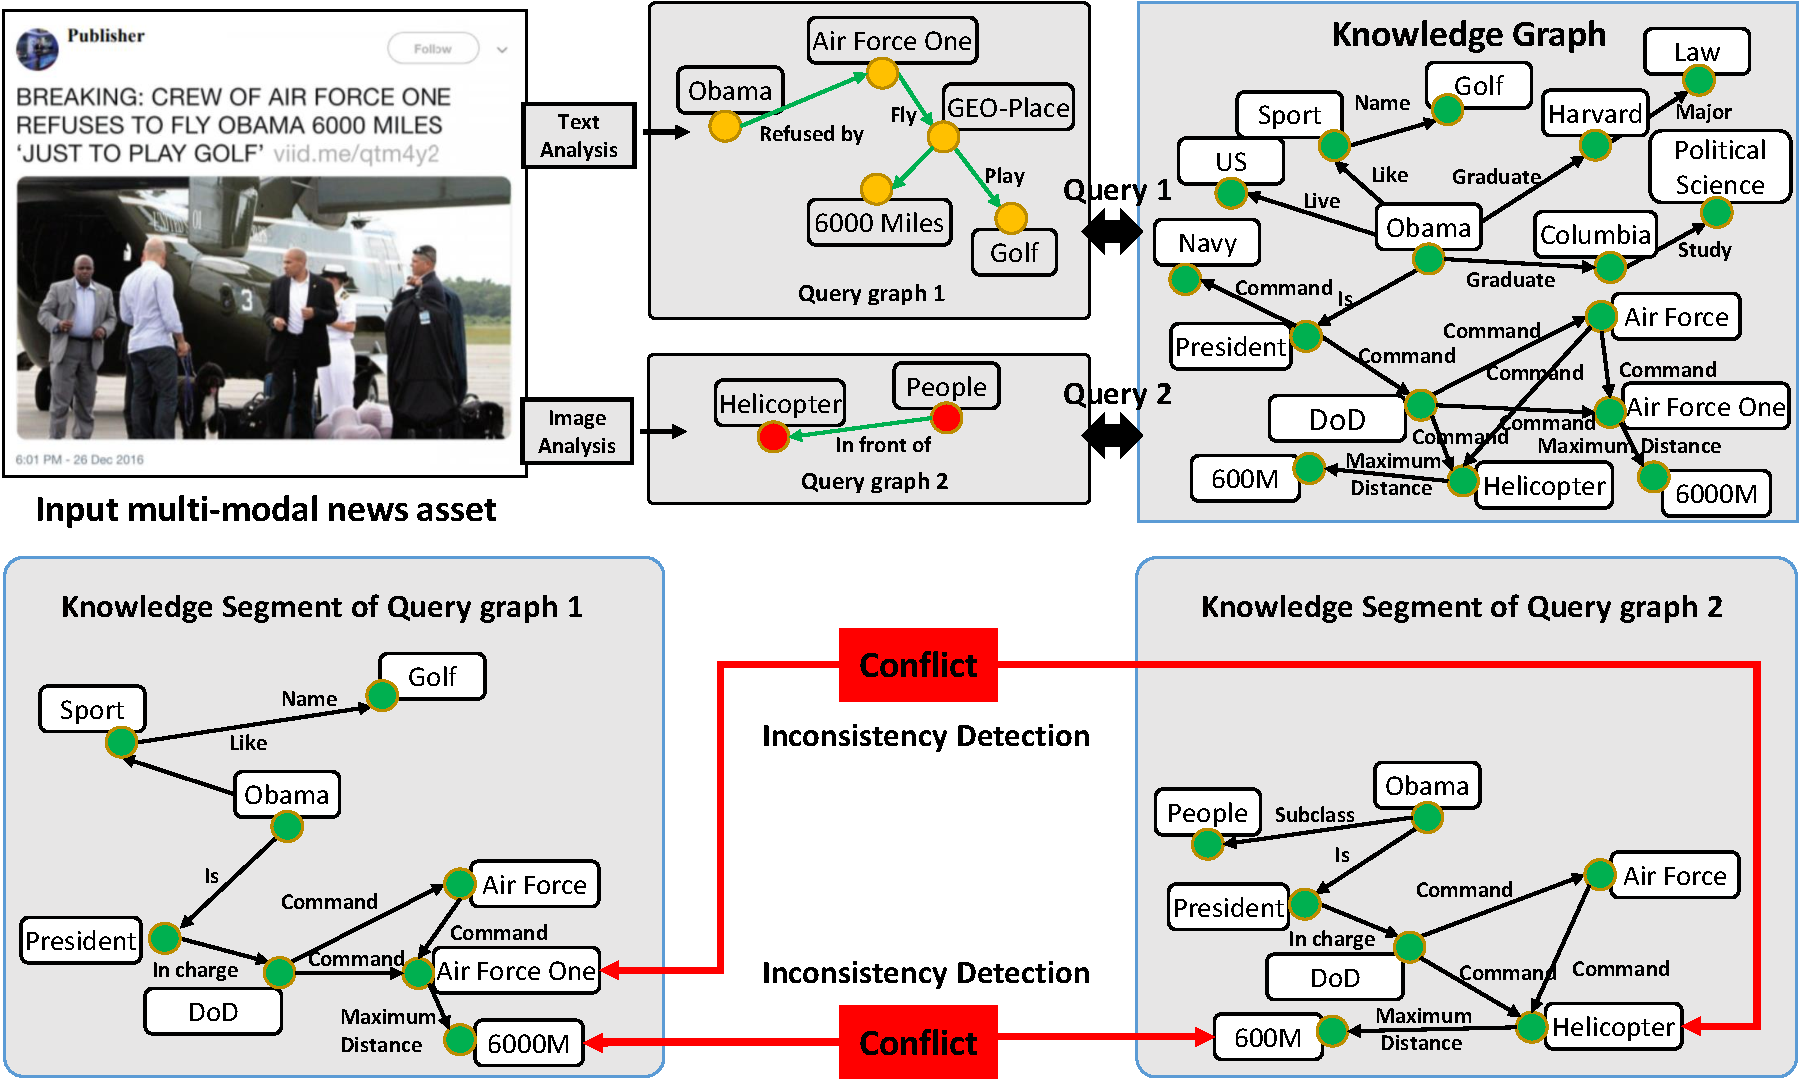
\includegraphics[width=0.8\textwidth]{submissions/logical-queries-uiuc/img/pdfresizer.pdf}
\caption{An illustrative example of using comparative reasoning for semantic inconsistency detection. Source of the image at the top-left: \cite{Cui2019SAMES}. The example is borrowed from ~\cite{kompare}.
}
\label{inconsistency}
\end{figure*}


%\section{Problem Definition}

%\input{002probDef.tex}

%\subsection{Knowledge Graph Search}
%\input{002probDef01match.tex}
%\subsection{Knowledge Graph Reasoning}
%\input{002probDef02Reason.tex}

\section{Problem Definition}\label{problem_definition}



\hide{
\begin{table}[]
	\centering
	\footnotesize
	\caption{Notations and definitions}
	\begin{tabular}{|c|c|}
		\hline
		{\bf Symbols}       & {\bf Definition}                \\ \hline
		$\mathcal{G}$=\{$V^G$, $E^G$, $L^G$\} & a knowledge graph  \\ \hline
		$v_i$         & the $i^\textrm{th}$ entity/node in knowledge graph \\ \hline
		$r_i$         & the $i^\textrm{th}$ relation/edge in knowledge graph \\ \hline
		$e_i$         & the $i^\textrm{th}$ given by the user   \\ \hline
		$KS_i$         & knowledge segment $i$ \\ \hline
		${Q}$=\{$V^Q$, $E^Q$, $L^Q$\} & an attributed query graph \\ \hline
		$A_i$         & adjacency matrix of $KS_i$ \\ \hline
		$N_i$         & {attribute matrix of $KS_i$, the $j^\textrm{th}$ row} \\  
		 ~ & {denotes the attribute vector of node $j$ in $KS_i$} \\ \hline
		$A_{\times}$      & kronecker product of $A_1$ and $A_2$      \\ \hline
		$N^l$      & diagonal matrix of the $l^\textrm{th}$ node attribute  \\ \hline
		$N_{\times}$      &  combined node attribute matrix  \\ \hline
		$S^{i,j}$          & single entry matrix $S^{i,j}(i,j)=1$ and zeros elsewhere  \\ \hline
	\end{tabular}
\label{notation}
\vspace{-1.5\baselineskip}
\end{table}
}


\begin{table}[]
	\centering
	\footnotesize
	\caption{Notations and definitions}
	\setlength\tabcolsep{1.5pt}
	\begin{tabular}{|c|c|c|c|}
		\hline
		{\bf Symbols}       & {\bf Definition}     & {\bf Symbols}       & {\bf Definition}              \\ \hline
		$\mathcal{G}$=\{$V^G$, $E^G$, $L^G$\} & a knowledge graph  & $v_i$         & the $i^\textrm{th}$ entity/node in knowledge graph \\ \hline
		$r_i$         & the $i^\textrm{th}$ relation/edge in knowledge graph & $e_i$         & the $i^\textrm{th}$ given by the user   \\ \hline
		
		${Q}$=\{$V^Q$, $E^Q$, $L^Q$\} & an attributed query graph &  $KS_i$         & knowledge segment $i$  \\ \hline
		
		$A_i$         & adjacency matrix of $KS_i$   &  $A_{\times}$      & kronecker product of $A_1$ and $A_2$      \\ \hline
		$N^l$      & diagonal matrix of the $l^\textrm{th}$ node attribute  & $N_{\times}$      &  combined node attribute matrix  \\ \hline
		
		
		$N_i$         & {attribute matrix of $KS_i$, the $j^\textrm{th}$ row} &  $S^{i,j}$          & single entry matrix $S^{i,j}(i,j)=1$ and zeros elsewhere  \\ 
		 ~ & {denotes the attribute vector of node $j$ in $KS_i$} & & \\ \hline
		
	\end{tabular}
\label{notation}
\end{table}

In this section, we  first introduce the  symbols that will be used throughout the paper, then we introduce other important concepts and formally define the comparative reasoning problem.

Table ~\ref{notation} gives the main notations used throughout this paper. 
A knowledge graph can be denoted as $\mathcal{G}=(V, R, E)$ where $V = \{v_1, v_2, ..., v_n\}$ is the set of nodes/entities, $R = \{r_1, r_2, ..., r_m\}$ is the set of relations and $E$ is the set of triples.
Each triple in the knowledge graph can be denoted as $(h, r, t)$ where $h \in V$ is the head (i.e., subject) of the triple, $t \in V$ is the tail (i.e., object) of the triple and $r \in R$ is the edge (i.e., relation, predicate) of the triple which connects the head $h$ to the tail $t$. 

Given multiple pieces of clues, the goal of comparative reasoning is to infer commonality and/or inconsistency among them.  
If the given information is a pair of clues, we call it pairwise comparative reasoning or pairwise fact checking. The goal is to deduce whether these two clues are coherent or not. 
If the given information is a connected query graph, the goal is to detect whether there is inconsistency inside the given graph. The problem is called collective comparative reasoning or collective fact checking.
Different from traditional point-wise reasoning methods, comparative reasoning can unveil some subtle patterns which point-wise approaches may overlook.
Take knowledge graph based fact checking as an example, considering two claims/triples: 
({\tt Barack Obama}, {\tt graduatedFrom}, {\tt Harvard University}) and
({\tt Barack Obama}, {\tt majorIn}, {\tt Political Science}).
Even each clue/claim is true,  but if we check them together at the same time, we can see that they cannot be both true. This is because {\tt Barack Obama} majored in {\tt law} instead of {\tt Political Science} when he studied at {\tt Harvard University}. So, we might fail to detect the inconsistency between them without appropriately examining different clues/claims together.

To facilitate comparative reasoning, how to utilize the background information in knowledge graph is an important problem.
If we can find a subgraph in the knowledge graph which can best express the semantic meaning of each input clue, the hidden conflicts can be easier to detect. Ideally, this subgraph should contain all the meaningful/important entities and relations in the knowledge graph which 
are related to the given clue.
We call this subgraph {\em knowledge segment}, 
which is formally defined as follows.
\begin{definition}{\textbf{Knowledge Segment (KS for short)}} is a connection subgraph of the knowledge graph that best describes the semantic context of a piece of given clue (i.e., a node, a triple or a query graph).\vspace{-0.5\baselineskip}
\end{definition}

Figure ~\ref{inconsistency} gives an example of { knowledge segment}. Given two clues which are two query graphs extracted from the text and image respective, their corresponding knowledge segments are shown in the bottom of the Figure. As we can see, expressing the given clues with { knowledge segments} can help us detect the inconsistency without difficulty. 


%When reasoning among multiple pieces of clues according to their knowledge segments, 

Given the knowledge segments of multiple pieces of clues,
comparative reasoning aims to infer the commonality and inconsistency among these knowledge segments to make decision.
For pairwise case, the commonality refers to the common elements of these two knowledge segments. The inconsistency includes any elements that are contradicts with each other. 
Assuming the two given clues are two edges/triples: $E^Q_1 = <{\tt s_1}, {\tt p_1}, {\tt o_1}>$ and $E^Q_2 = <{\tt s_2}, {\tt p_2}, {\tt o_2}>$ where ${\tt s_1}, {\tt o_1}, {\tt s_2}, {\tt o_2} \in V$ and ${\tt p_1}, {\tt p_2} \in E$. We denote their corresponding knowledge segments as $KS_1$ for $E^Q_1$ and $KS_2$ for $E^Q_2$, respectively. 
The commonality and inconsistency between these two knowledge segments are defined as follows. 
\begin{definition}{\textbf{Commonality.}}
Given two triples ($E^Q_1$ and $E^Q_2$) and their knowledge segments ($KS_1$ and $KS_2$), the commonality of these two triples refers to the shared nodes and edges between $E^Q_1$ and $E^Q_2$, as well as the shared nodes and edges between $KS_1$ and $KS_2$: $((V^{KS_1} \cap V^{KS_2}) \cup (V^{Q_1} \cap V^{Q_2}) , (E^{KS_1} \cap E^{KS_2}) \cup (E^{Q_1} \cap E^{Q_2})  )$.
\end{definition}
\vspace{-0.8\baselineskip}
\begin{definition}{\textbf{Inconsistency.}}
Given two knowledge segments $KS_1$ and $KS_2$, 
the inconsistency between these two knowledge segments refers to any element (node, node attribute or edge) in $KS_1$ and $KS_2$ that contradicts with each other. 
\end{definition}

Different from pairwise comparative reasoning, collective comparative reasoning aims to find the commonality and/or inconsistency inside a query graph which consists of a set of inter-connected edges/triples. The corresponding definition is given below.
\begin{definition}{\textbf{Collective Commonality.}}
For each edge $E^Q_i$ in a query graph $Q$, let $KS_i$ be its knowledge segment. % extracted from the knowledge graph. 
The collective commonality between any triple pair in the query graph is the intersection of their knowledge segments.
\end{definition}
\vspace{-0.8\baselineskip}
\begin{definition}{\textbf{Collective Inconsistency.}}
For each edge $E^Q_i$ in a query graph $Q$, let $KS_i$ be its knowledge segment. % extracted from the knowledge graph. 
The collective inconsistency refers to any elements (node or edge or node attribute) in these knowledge segments that contradict with each other.
\end{definition}


%Multi-pieces comparative reasoning aims at checking whether multiple pieces of clues are inconsistent. 
Given the above notation and information, the problem of comparative reasoning is formal defined as: 

\begin{pro-stat}{Pairwise Comparative Reasoning: }
	
	\textbf{Given:} (1) A knowledge graph $\mathcal{G}$, (2) two triples $E^Q_1$ and $E^Q_2$;
	
	\textbf{Output:} A binary decision regarding the consistency of $E^Q_1$ and $E^Q_2$.
	
\end{pro-stat}




\begin{pro-stat}{Collective Comparative Reasoning: }
	
	\textbf{Given:} (1) A knowledge graph $\mathcal{G}$, (2) a query graph ${Q}$;
	
	\textbf{Output:}  A binary decision regarding the consistency of ${Q}$.
	
\end{pro-stat}







\section{Knowledge Segment Extraction}\label{ks_extractt}

%



In this section, we introduce how to extra knowledge segment to best express the semantic meaning of a given claim. We first introduce how to transform the knowledge graph into a relation specified weighted graph, then introduce how to extract Edge-specific Knowledge Segment and Subgraph-specific Knowledge Segment from it.


Generally speaking, given a clue (e.g., a triple or a query graph) from the user, 
the goal of knowledge segment extraction is to extra a subgraph which can best express the semantic meaning of the given clue.
Many existing methods have been proposed to  extract a concise subgraph from the source node of the querying edge to its target node in weighted or unweighted graphs. For example, multi-hop method ~\cite{knowledge-path}, minimum cost maximum flow method ~\cite{Shiralkar2017}, {\em K-}simple shortest paths based method ~\cite{Freitas} or connection subgraph  ~\cite{Faloutsos2004}, ~\cite{Koren2006MEP}, ~\cite{conan} extraction methods.


However, these methods do not directly apply to knowledge graphs because the edges (i.e., predicates) of a knowledge graph have specific semantic meanings (e.g., types, relations). To address this issue, we seek to convert the knowledge graph to a weighted graph by designing a predicate-predicate similarity measure for knowledge segment extraction. 


\subsection{Predicate-Predicate Similarity}

In order to transform the knowledge graph into weighted graph, 
We propose to use a TF-IDF based method to measure the similarity between different predicates, and transfer the knowledge graph into a weighted graph whose edge weight represents the similarity between the edge predicate and query predicate. 
The key idea behind TF-IDF based method is that we can treat each triple in the knowledge graph and its adjacent neighboring triples as a document, and use a TF-IDF like weighting strategy to calculate the predicate similarity. For example, predicate ${\tt receiveDegreeFrom}$ may have neighbor predicates $ {\tt major}$ and ${\tt graduateFrom}$. These predicates should have high similarity with each other. 

To be specific, we use the knowledge graph to build a co-occurrence matrix of predicates, and calculate their similarity by a TF-IDF like weighting strategy as follows. Let $i,j$ denote two different predicates. We define the $\textrm{TF}$ between two predicates as $\textrm{TF}(i, j) = \log(1 + C(i,j) {w}(j))$, where $C(i,j)$ is the co-occurrence of predicate $i$ and $j$. The $\textrm{IDF}$ is defined as $\textrm{IDF}(j) = \log \frac{|M|}{|\{i : C(i,j)>0\}|}$, 
where $M$ is the number of predicates in the knowledge graph. Then, we build a TF-IDF weighted co-occurrence matrix $U$ as $U(i, j) = \textrm{TF}(i, j) \times IDF(j)$.
Finally, the similarity of two predicates is defined as $\textrm{Sim(i, j)} = \textrm{Cosine}(U_i, U_j)$, 
where $U_i$ and $U_j$ are the $i^{th}$ row and $j^{th}$ row of $U$, respectively.

For the predicate-predicate similarity,
suppose we want to calculate the similarity between {\tt major} and {\tt study}. Both {\tt major} and {\tt study}  have only one adjacent neighboring predicate {\tt graduate}. This means that for any predicate $i \neq {\tt graduate}$, $U({\tt major}, i) = U({\tt study}, i) = 0$.
Since $\textrm{E}({\tt graduate}) = 0$, we have ${w}({\tt graduate}) = 2\sigma(\infty) - 1 = 1$. We have \textrm{TF}({\tt major}, {\tt graduate}) = \textrm{TF}({\tt study}, {\tt graduate}) = $\log(1 + 1 \times 1) = 1$, and $U({\tt major}, {\tt graduate}) = U({\tt study}, {\tt graduate}) = IDF({\tt graduate}) = \log\frac{8}{4} = 1$. If we compare the two vectors, $U_{{\tt major}}$ and $U_{{\tt study}}$, we find that they are the same. Therefore, we have that $\textrm{Sim}({\tt major}, {\tt study}) = 1$.


\subsection{Edge-specific Knowledge Segment}~\label{basic:edge}\vspace{-1\baselineskip}

Edge-specific knowledge segment extraction aims at finding a knowledge segment to best characterize the semantic context of the given edge (i.e., a triple). 
Several connection subgraph extraction methods exist for a weighted graph, e.g., ~\cite{Tong2006CSP} uses a random walk with restart based method to find an approximate subgraph; ~\cite{Koren2006MEP} uses maximal network flow to find a subgraph and ~\cite{Freitas} aims to find a denser local graph partitions. In this paper,
after transforming the knowledge graph into a weighted graph, we find {\em k-}simple shortest paths~\cite{Koren2006MEP} from the subject to the object of the given query edge as its knowledge segment. 



\subsection{Subgraph-specific Knowledge Segment}~\label{basic:subgraph}

Following the idea of edge-specific knowledge segment extraction, we extract a knowledge segment for each edge in the given subgraph and we call the graph which contains all the edge-specific knowledge segments subgraph-specific knowledge segment.
In other words, a subgraph-specific knowledge segment consists of multiple inter-linked edge-specific knowledge segments (i.e., one edge-specific knowledge segment for each edge of the input query subgraph). 

The subgraph-specific knowledge segment provides richer semantics, including both the semantics for each edge of the query graph and the semantics for the relationship between different edges of the input query graph. 








%\input{004search.tex}

\section{Comparative Reasoning}\label{methods}

In this section, we introduce the technical details behind comparative reasoning.
We first introduce on what condition we need to exert pairwise reasoning for two pieces of clues (e.g., two edges/triples),
and then introduce two methods which focus on pairwise reasoning.
Finally, we present the collective comparative reasoning.
The main idea behind these functions is that we use a knowledge segment to express the semantic meaning of each query triple, and
check the inconsistency according to information in the knowledge segments.


\subsection{Pairwise Comparative Reasoning Condition}

%Given a pair of triples, we may don't need to check them if they talk about different things.
Given a pair of clues $<{\tt s_1}, {\tt p_1}, {\tt o_1}>$ and $<{\tt s_2}, {\tt p_2}, {\tt o_2}>$, we can divide it into the following six cases, including
\noindent
\begin{enumerate}[wide, labelwidth=!, labelindent=0pt]
\item [C1.]
{
${\tt s_1} \neq {\tt s_2}$, ${\tt s_1} \neq {\tt o_2}$, ${\tt o_1} \neq {\tt s_2}$, ${\tt o_1} \neq {\tt o_2}$.
For this case, these two clues apparently refer to different things,
e.g., $<${\tt Alan Turing}, {\tt wasBornIn}, {\tt United Kingdom}$>$ and $<${\tt Google}, {\tt isLocatedIn}, {\tt USA}$>$.
}
\item [C2.]
{
%Given $<{\tt s_1}, {\tt p_1}, {\tt o_1}>$ and $<{\tt s_2}, {\tt p_2}, {\tt o_2}>$, where
${\tt s_1} = {\tt s_2}$ and ${\tt o_1} = {\tt o_2}$.
If ${\tt p_1} = {\tt p_2}$, these two clues are the same.
If ${\tt p_1}$ and ${\tt p_2}$ are different or irrelevant, e.g., ${\tt p_1} ={\tt wasBornIn}$, ${\tt p_2} = {\tt hasWebsite}$,
these two clues refer to different things.
However, if ${\tt p_1}$ contradicts ${\tt p_2}$, they are inconsistent with each other.
}
\item [C3.]
{
%Given $<{\tt s_1}, {\tt p_1}, {\tt o_1}>$ and $<{\tt s_2}, {\tt p_2}, {\tt o_2}>$, where
${\tt s_1} = {\tt s_2}$ but ${\tt p_1} \neq {\tt p_2}$ and ${\tt o_1} \neq {\tt o_2}$, e.g., $<${\tt Alan Turing}, {\tt wasBornIn}, {\tt Maida Vale}$>$, $<${\tt Alan Turing}, {\tt livesIn}, {\tt United Kingdom}$>$.
}
\item [C4.]
{
%Given $<{\tt s_1}, {\tt p_1}, {\tt o_1}>$ and $<{\tt s_2}, {\tt p_2}, {\tt o_2}>$, where
${\tt s_1} = {\tt s_2}$, ${\tt p_1} = {\tt p_2}$, but ${\tt o_1} \neq {\tt o_2}$,
e.g., $<${\tt Alan Turing}, {\tt wasBornIn}, {\tt Maida Vale}$>$, $<${\tt Alan Turing}, {\tt wasBornIn}, {\tt United Kingdom}$>$.
}
\item [C5.]
{
%Given $<{\tt s_1}, {\tt p_1}, {\tt o_1}>$ and $<{\tt s_2}, {\tt p_2}, {\tt o_2}>$, where
${\tt o_1} = {\tt o_2}$, but ${\tt s_1} \neq {\tt s_2}$.
For this case, no matter what ${\tt p_1}$ and ${\tt p_2}$ are, these two clues refer to different things.
}
\item [C6.]
{
%Given $<{\tt s_1}, {\tt p_1}, {\tt o_1}>$ and $<{\tt s_2}, {\tt p_2}, {\tt o_2}>$, where
${\tt o_1} = {\tt s_2}$.
For this case, no matter what ${\tt p_1}$ and ${\tt p_2}$ are, they refer to different things.
For example, $<${\tt Alan Turing}, {\tt wasBornIn}, {\tt United Kingdom}$>$, $<${\tt United Kingdom}, {\tt dealsWith}, {\tt USA}$>$.
}
\end{enumerate}


%\vspace{-1\baselineskip}
Among these six cases, we can see that the clue pair in C1, C5 and C6 refer to different things. Therefore, there is no need to check the inconsistency between them. For C2, we only need to check the semantic meaning of their predicates, i.e., whether ${\tt p_1}$ contradicts ${\tt p_2}$. For example, ${\tt p_1} = {\tt isFather}$ and ${\tt p_2} = {\tt isSon}$, they are inconsistent with each other. Otherwise, there is no inconsistency between them.
%\hh{add details: e.g. if p1 is the opposite of p2, they are inconsistent. otherwise, there is no inconsistency.}.
We mainly focus on C3 and C4 where the two clues may be inconsistent with each other even if each of them is true. For example,
%in Figure ~\ref{inconsistency},
either $<${\tt Barack Obama}, {\tt graduatedFrom}, {\tt Harvard University}$>$ or $<${\tt Barack Obama}, {\tt majorIn} , {\tt Political Science}$>$
could be true. But putting them together, they cannot be both true, since
{\tt Barack Obama} majored in {\tt law} instead of {\tt Political Science} when he studied at {\tt Harvard University}.
%these two claims could not happen at the same time.
In other words, they are mutually exclusive with each other and thus are inconsistent.
However,
queries like $<${\tt Alan Turing}, {\tt wasBornIn}, {\tt Maida Vale}$>$ and $<${\tt Alan Turing}, {\tt wasBornIn}, {\tt United Kingdom}$>$ are both true, because {\tt Maida Vale} belongs to {\tt United Kingdom}. Alternatively, we can say that {\tt United Kingdom} contains {\tt Maida Vale}.
We summarize that if (1) the subjects of two clues are the same, and (2) their predicates are similar with each other or the same, they refer to the same thing. Furthermore, if their objects are two uncorrelated entities, it is highly likely that these two clues are inconsistent with each other.

Based on the above observations, we take the following three steps for pairwise comparative reasoning. First, given a pair of clues, we decide which of six cases it belongs to, by checking the subjects, predicates and objects of these two clues. Second, if this pair of clues belongs to C3 or C4, we need to further decide whether they are consistent with each other. In the following sections, we illustrate how to tackle this case.

\subsection{Neural Network Based Pairwise Comparative Reasoning}

Given two knowledge segments of a pair of clues which belong to C3 or C4,
we treat each knowledge segment as an attributed graph, and adopt some ideas from network alignment to facilitate comparative reasoning.
The basic idea is that if the two knowledge segments are consistent, most of their nodes must be able to align with or close to each other in the embedding space. Otherwise, the embedding distance of the inconsistent nodes should be large.
Generally, the inconsistent checking problem is similar to anomaly detection or dissimilarity detection problem in the embedding space.

When reasoning a pair of knowledge segments, we consider two kinds of information: structure information and semantic information. We envision that both of them are important. For example, in Figure ~\ref{inconsistency}, {\tt Air Force One} and {\tt Helicopter} have similar structure information because they have many common neighbors, but their semantic meanings are very different, this may indicate a potential inconsistency between the two knowledge segments. On the other hand, although {\tt Air Force One} and {\tt Helicopter} have different structure information (when considering edge type), they also have different semantic information. This prompts that they refer to the different things. Inspired by this observation, we propose a neural network model which considers both the structure information and semantic information of knowledge segments to achieve pairwise comparative reasoning.



To encode the structure similarity, we use random walk with restart (considering edge type) to encode the knowledge segment structure information. The similar idea has been used by many other works, e.g. ~\cite{Tong2006rdwalk}, ~\cite{bright}.
Given a set of anchor nodes, random walk with restart will calculate a score for each node in the knowledge segment w.r.t. each anchor node. If two nodes have the similar random walk with restart score vector, their structure similarity should be high.
To encode the semantic information of the knowledge segment, we borrow some ideas from natural language processing. More specifically, we sample some paths from the knowledge graph, and treat each path as a sentence, nodes in the knowledge graph can be treated as words in the sentence. If two nodes occur in the same sentence, their semantic information should be similar.


\subsubsection{Structure Embedding}

Given two knowledge segments, the common nodes in these two knowledge segments can be treated as anchor entities, structure embedding
aims to embed the nodes in the knowledge segments to a high dimension space while keeping their structure information.
The key intuition is that, the set of anchor links $\mathcal{L}$ provides the landmarks for all nodes in both networks. Relative positions based on anchor links can form a unified space for all nodes regardless which network they belong to ~\cite{bright}. Therefore, we can use random walk with restart to measure the relative position between nodes and anchor links.
Let $KS_1$ and $KS_2$ be the two knowledge segments.
Given an anchor link $l \in \mathcal{L}$ (we use $l_1$ and $l_2$ to denote the linked entities in $KS_1$ and $KS_2$),
the $\textrm{RWR}$ score vector $r_{l_1}$ of size $n_1 \times 1$ can be obtained
\begin{equation}
r_{l_1} = (1 - \beta)\hat{W_1} r_{l_1} + \beta e_{l_1}
\end{equation}
where $n_1$ is the number of nodes in $KS_1$, $\hat{W_1}$ is the row normalized adjacency matrix of $KS_1$, $\beta$ is the restart probability and $e_{l_1}$ is one-hot vector with  $e_{l_1}(l_1) = 1$ and all other entries are 0.
We can solve the equation and get the final expression of $r_{l_1}$ as:
\begin{equation}
r_{l_1} = \beta (I - (1 - \beta))\hat{W_1}^{-1} e_{l_1}
\end{equation}
Note that if $KS_1$ and $KS_2$ are the same, they will have the same random walk with restart score matrices.

After we get the  random walk with restart matrices, we then use a share neural network to learn the embedding of these two knowledge segments. In this way, the structure information of each node can be kept in the embedding space. The learned embedding for $KS_1$ can be calculated as:
\begin{equation}
E_{1} = \textrm{NeuralNetwork}(\textrm{RWR}_{1})
\end{equation}
where $\textrm{RWR}_{1}$ is the random walk with restart score matrix of $KS_1$. $\textrm{RWR}_{2}$ can be calculated in the same way.

\subsubsection{Semantic Embedding}

To captivate the semantic meaning of each node in the knowledge segment, we randomly sample some paths in the background knowledge graph and treat each path as an utterance while each node as a word in the sentence. Then, we use a popular language model Bert ~\cite{bert} to learn the semantic embedding of each node. If two nodes occur at the same path, their semantic embedding should be close to each other, otherwise, their semantic embedding should be far from each other.


We concatenate the node semantic embedding and structure embedding of two knowledge segments and use graph neural network to learn the graph embedding of $KS_1$ and $KS_2$ respectively. Finally, we predict whether they are consistent with each other according to the graph embedding. The architecture of the algorithm is shown in Figure ~\ref{nn_pairwise}.


\begin{figure*}[ht!]
\centering
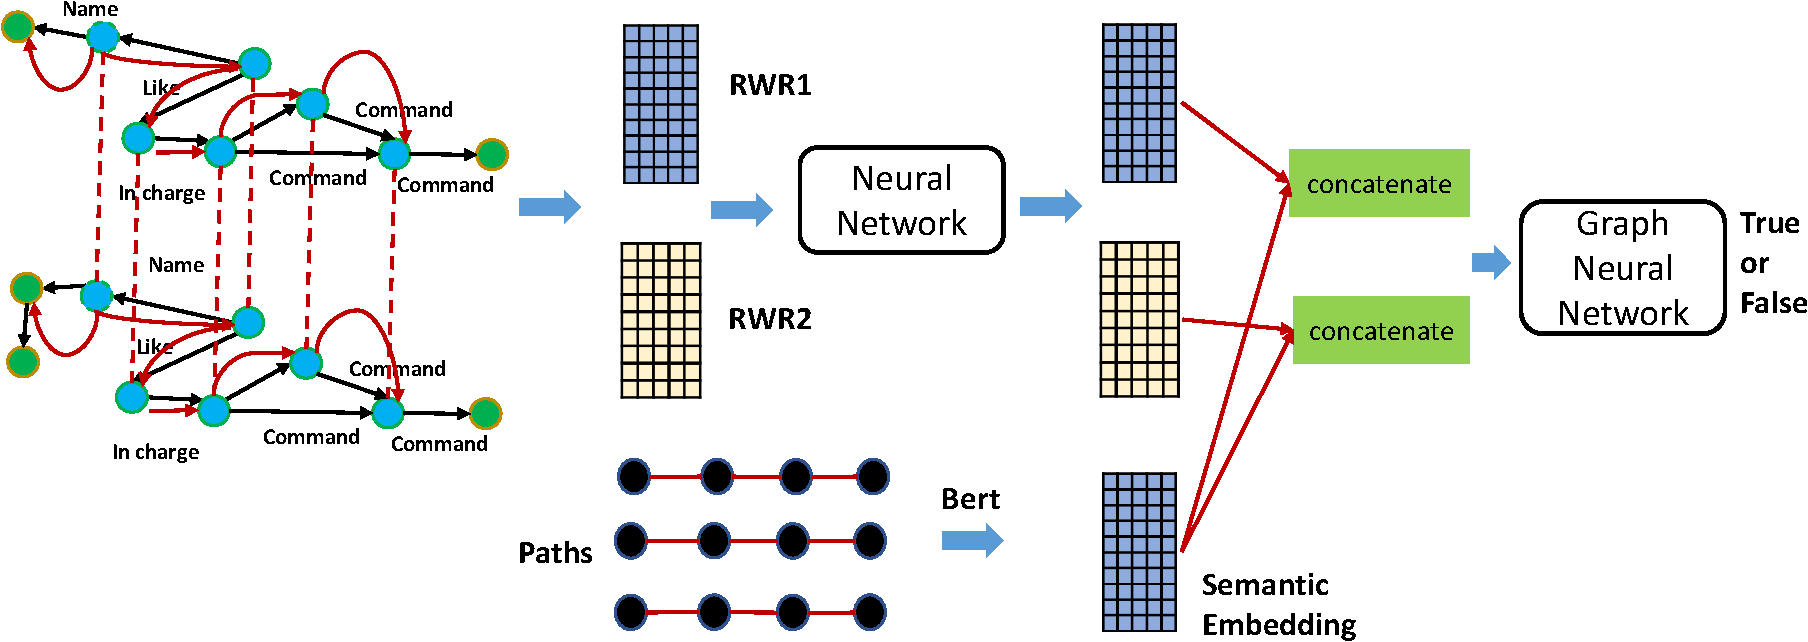
\includegraphics[width=0.9\textwidth]{submissions/logical-queries-uiuc/img/nn_pairwise_reasoning.pdf}
\caption{Neural network based pairwise comparative reasoning framework.
}
\label{nn_pairwise}
\end{figure*}

The pseudo code is given in Algorithm~\ref{pair_nn}. GNN means graph neural network which is defined as follows
\begin{equation}
    x^l_{N(u)} = \textrm{AGGREGATE}(\{\mathbf{X}^l(v,:), for v\in N(u)\})
\end{equation}
\begin{equation}
    \mathbf{X}^{l+1}(u,:) = \sigma(\textrm{CONCAT}(\mathbf{X}^l(u,:), x^l_{N(u)}))
\end{equation}
where AGGREGATE is the aggregation function, $\mathbf{X}$ is the input node embedding, $l$ is the graph neural network layer number, and $(u, v)$ are nodes in the input graph. The classifier in Algorithm~\ref{pair_nn} can be any machine learning model, e.g., SVM, logistic regression, decision tree and so on.

\begin{algorithm}[H] % algorithm begin
	\caption{Neural Network Based Pairwise Comparative Reasoning} % Algorithm title
	\label{pair_nn}
	\begin{algorithmic}[1]
		\STATE \textbf{Input:} Knowledge segment $KS_1$ and knowledge segment $KS_2$, pretrained embedding of all entities $\mathbf{E}$ in the knowledge graph.
		\STATE \textbf{Training:}
		\STATE Calculate random walks with restart matrices $\textrm{RWR}_1$  and $\textrm{RWR}_2$ for $KS_1$ and  $KS_2$, respectively.
		\STATE $E_{1}$ = NeuralNetwork($\textrm{RWR}_{1}$)
		\STATE  $E_{2}$ = NeuralNetwork($\textrm{RWR}_{2}$)
		\STATE Get all node embedding in $KS_1$: $N_{1}$ = $\mathbf{E}(KS_1)$
		\STATE Get all node embedding in $KS_2$: $N_{2}$ = $\mathbf{E}(KS_2)$
  	\STATE Concatenate embedding $C_1 = (E_{1} | N_{1})$
        \STATE Concatenate embedding $C_2 = (E_{2} | N_{2})$
        \STATE Predict result: Classifier(GNN($C_1$), GNN($C_2$))
	\end{algorithmic}
\end{algorithm}
\vspace{-1\baselineskip}

\subsection{Graph Kernel Based Pairwise Comparative Reasoning}

Different from neural network based pairwise comparative reasoning, graph kernel based pairwise comparative reasoning aims to utilize graph kernel to find a set of key elements (nodes or edges or node attributes) in these two knowledge segments and then make decision according to these elements and related information in the knowledge graph.
The idea is that if most of these key elements belong to the commonality of these two knowledge segments, it is highly likely that they refer to the same thing. Otherwise, these two clues refer to different things. Third, if they refer to the same thing, we further decide whether they conflict with each other. Here, the key idea is as follows. We build two new query triples $<{\tt o_1}$, {\tt isTypeOf}, ${\tt o_2}>$ and $<{\tt o_2}$, {\tt isTypeOf}, ${\tt o_1}>$. If one of them is true, the original two triples are consistent with each other. Otherwise, they are inconsistent.

In order to find the key elements, we propose to use the influence function w.r.t. the knowledge segment similarity \cite{qinghai}. The basic idea is that if we perturb a key element (e.g., change the attribute of a node or remove a node/edge), it would have a significant impact on the overall similarity between these two knowledge segments. Let $KS_1$ and $KS_2$ be the two knowledge segments.
We can treat the knowledge segment as an attributed graph, where different entities have different attributes.
We use random walk graph kernel with node attribute to measure the similarity between these two knowledge segments ~\cite{qinghai} ~\cite{sysvester}.

\vspace{-1\baselineskip}
\begin{eqnarray}\label{eq:rwgraphkernel}
\textrm{Sim}(KS_1, KS_2) = q'_{\times}(I - cN_{\times}A_{\times})^{-1}N_{\times}p_{\times}
\end{eqnarray}
where ${q'}_{\times}$ and $p_{\times}$ are the stopping probability distribution and the initial probability distribution of random walks on the product matrix, respectively. $N_{\times}$ is the combined node attribute matrix of the two knowledge segments $N_{\times} = \sum_{j=1}^d N_1^j \otimes N_2^j$ where $N_i^j$ ($i\in \{1,2 \}$) is the diagonal matrix of the $j^\textrm{th}$ column of attribute matrix $N_i$.
$A_{\times}$ is the Kronecker product of the adjacency matrices of knowledge segments $A_1$ and $A_2$. $0 < c < 1$ is a parameter.

We propose to use the influence function $\textrm{Sim}(KS_1 , KS_2)$ w.r.t. knowledge segment elements
 $\frac{\partial{Sim(KS_1, KS_2)}}{\partial {e}}$,
where $e$ represents an element of the knowledge segment $KS_1$ or $KS_2$.
The element with a high absolute influence function value is treated as a key element, and it can be a node, an edge, or a node attribute.
The influence function of different elements can be computed according to the following lemma.
Note that the influence function w.r.t. elements in $KS_2$ can be computed in a similar way.
\vspace{-0.3\baselineskip}
\begin{lemma}\label{lm:influence}\noindent (Knowledge Segment Similarity Influence Function ~\cite{qinghai}.)
Given $\textrm{Sim}(KS_1, KS_2)$
in Eq.~\eqref{eq:rwgraphkernel}.
Let $Q = (I - c N_{\times} A_{\times})^{-1}$ and $S^{j,i}$ is a single entry matrix defined in Table~\ref{notation}.
We have that
\item [] (i) The influence of an edge $A_1(i,j)$ in $KS_1$ can be calculated as
\begin{equation}
    I(A_1(i,j))= \frac{\partial \textrm{Sim}(KS_1, KS_2)}{\partial A_1(i,j)} =
c {q'}_{\times}QN_{\times}[(S^{i,j} + S^{j,i})\otimes A_2]QN_{\times}p_{\times}
\end{equation}


\item [] (ii) The influence of a node $i$ in $KS_1$ can be calculated as
\begin{equation}
    I(N_1(i)) = \frac{\partial \textrm{Sim}(KS_1, KS_2)}{\partial N_1(i)} =
c {q'}_{\times}QN_{\times}[\sum_{j|A_1(i,j)=1}(S^{i,j} + S^{j,i})\otimes A_2]QN_{\times}p_{\times}
\end{equation}


\item [] (iii) The influence of a node attribute $j$ of node $i$ in $KS_1$ can be calculated as
\begin{equation}
    I(N_1^j(i, i)) = \frac{\partial \textrm{Sim}(KS_1, KS_2)}{\partial N_1^j(i, i)} =
q'_{\times}Q[S^{i,i}\otimes N_2^j](I + c A_{\times}QN_{\times})p_{\times}
\end{equation}


%\hh{(1) check if the equation are correct. (2) and if we need to explain additional notations.}
\end{lemma}
\vspace{-0.3\baselineskip}



For a given knowledge segment, we flag the top 50\% of the elements (e.g., node attribute, node and edge) with the highest absolute influence function values as key elements.
We would like to check whether these key elements belong to the commonality of these two knowledge segments. If most of them (e.g., 60\% or more) belong to the commonality of these two knowledge segments, we say the two query clues describe the same thing. Otherwise, they refer to different things and thus we do not need to check the inconsistency between them.

If we determine that the query clues refer to the same thing, the next step is to decide whether they are inconsistent with each other. That is, given query clues $<{\tt s_1}$, ${\tt p_1}$, ${\tt o_1}>$ and $<{\tt s_1}$, ${\tt p_2}$, ${\tt o_2}>$, we need to decide whether ${\tt o_1}$ belongs to ${\tt o_2}$ or ${\tt o_2}$ belongs to ${\tt o_1}$.
To this end, we build two new queries $<{\tt o_1}$, {\tt isTypeOf}, ${\tt o_2}>$ and $<{\tt o_2}$, {\tt isTypeOf}, ${\tt o_1}>$. Then, we extract the knowledge segments for these two queries, and check whether these two segments are true. If one of them is true, we say the original clues are consistent with each other, otherwise they are inconsistent.
After we extract the knowledge segments for $<{\tt o_1}$, {\tt isTypeOf}, ${\tt o_2}>$ and $<{\tt o_2}$, {\tt isTypeOf}, ${\tt o_1}>$, we treat each knowledge segment as a directed graph, and calculate how much information can be transferred from the subject to the object. We define the transferred information amount %\hh{let us use 'transferred information amount' consistently}
as:
\begin{equation}\label{eq:transinfo}
    \textrm{infTrans}({\tt o_1}, {\tt o_2}) = \max_{1 \leq j \leq k} \textrm{pathValue}(j)
\end{equation} where $\textrm{pathValue}(j)$ is defined as the multiplication of the weights in the path. For an edge, its weight is the predicate-predicate similarity $\textrm{Sim}({\tt isTypeOf}, e_i)$. If $\max\{\textrm{infTrans}({\tt o_1}, {\tt o_2}),  \textrm{infTrans}({\tt o_2}, {\tt o_1})\}$ is larger than a threshold $T$, then we say ${\tt o_1}$ belongs to ${\tt o_2}$ or ${\tt o_2}$ belongs to ${\tt o_1}$. We set $T = 0.700$ in our experiment.

\hide{
\begin{figure}
	\centering
	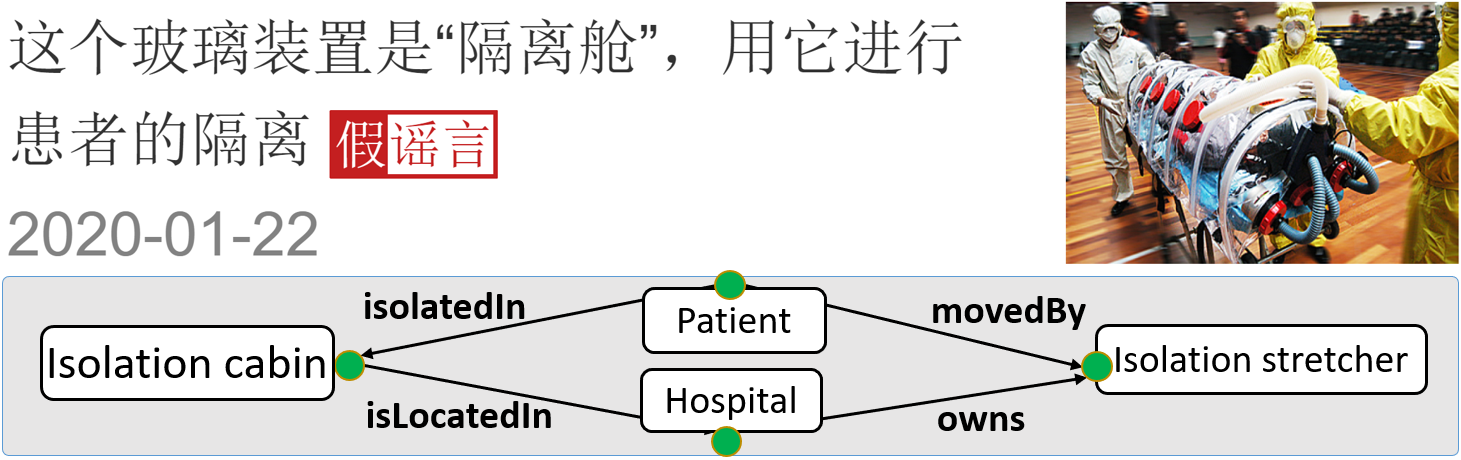
\includegraphics[width=0.43\textwidth]{img/qq_example.png}
	\vspace{-1\baselineskip}
	\caption{A fake news example from Wuhan coronavirus crisis. The text in the news says ``{\em This glass device is `Isolation Cabin', which is used to  isolate patients.}".}
	\label{qq_example}
	\vspace{-1\baselineskip}
\end{figure}


Let us take an example from Wuhan coronavirus crisis which is shown in Figure ~\ref{qq_example}.
The query we get from text is $<${\tt Patient}, {\tt isolatedIn}, {\tt Isolation Cabin}$>$,
and the query we get from image is $<${\tt Patient}, {\tt isolatedIn}, {\tt Isolation stretcher}$>$.
To detect the inconsistency of this pair of clues, we only need to check whether $<${\tt Isolation Cabin}, {\tt isTypeOf}, {\tt Isolation stretcher}$>$ or $<${\tt Isolation stretcher}, {\tt isTypeOf}, {\tt Isolation Cabin}$>$.
If we have $\textrm{infTrans}({\tt Isolation~Cabin}, {\tt Isolation~stretcher}) < 0.700$ based on the knowledge segment extracted from the knowledge graph, we conclude that Isolation Cabin is not Isolation stretcher. Therefore, there exists inconsistency in this news.% about Wuhan coronavirus crisis.
}

%%%%%%%%%%%%%%%%%%%%%%%%%%%%%%%%%%%%%%%%%%%%%%%%%%%%%%%%%%%%%%%%%%%%%%%%%%%%%%%%%%%%%%%%%%%%%%%%%%%%%%%%%%%%%%


\subsection{Graph Kernel Based Collective Comparative Reasoning}

%In last section, we introduce the pairwise comparative reasoning. In this section, we introduce collective comparative reasoning.
Different from pairwise comparative reasoning, collective comparative reasoning aims to find the commonality and/or inconsistency inside a query graph which consists of a set of inter-connected edges/triples.
To check the inconsistency, one naive method is using the pairwise comparative reasoning method to check the inconsistency for each pair of edges in the query graph. However, this method is neither computationally efficient nor sufficient. For the former, if two clues (e.g., two claims from a news article) are weakly or not related with each other on the query graph, we might not need to check the inconsistency between them at all. For the latter, in some subtle situations, the semantic inconsistencies could {\em only} be identified when we collectively reason over multiple (more than two) knowledge segments. For example, given the following three claims, including
(1) {\em Obama is refused by Air Force One};
(2) {\em Obama is the president of the US};
(3) {\em The president of US is in front of a helicopter}.
Only if we reason these three claims collectively, can we identify the semantic inconsistency among them.
%In other cases, the additional claim (e.g., <Marine One, max distance, 600M>) and its corresponding knowledge segment might provide extra corroborations for pairwise semantic inconsistency reasoning (e.g., <Obama, field, 6,000M> and <Obama, in front of, Marine One>).

%The idea behind collective comparative reasoning is that if the query graph is consistent, the semantic matching subgraph should contain no inconsistency.
Based on the above observation, we propose the following method to detect the collective inconsistency.%\bx{'First' goes to a new line?}

\textbf{First}, we find a set of key elements inside the semantic matching subgraph.
Different from pair-wise comparative reasoning, the importance/influence of an element for collective comparative reasoning is calculated by the entire semantic matching subgraph.
More specifically,
we first transform the query graph and its semantic matching subgraph (i.e., subgraph-specific knowledge segment) into two line graphs, which are defined as follows.
\vspace{-0.5\baselineskip}
\begin{definition} {\bf Line Graph~\cite{Shiralkar2017}}.
For an arbitrary graph $G=(V, E)$, the line graph $L(G) = (V', E')$ of  $G$ has the following properties:
(1) the node set of $L(G)$ is the edge set of $G$ ($V' = E$);
(2) two nodes $V'_i$, $V'_j$ in $L(G)$ are adjacent if and only if the corresponding edges $e_i$, $e_j$ of $G$ are incident on the same node in $G$.
\end{definition}
\vspace{-0.5\baselineskip}
Figure ~\ref{collective-compare-workflow} gives an example of the line graph.
For the line graph $L(Q)$, the edge weight is the predicate-predicate similarity of the two nodes it connects.
For the line graph $L(KS)$, the edge weight is the knowledge segment similarity by Eq.~\eqref{eq:rwgraphkernel} of the two nodes it connects.
The rationality of building these two line graphs is that if the semantic matching subgraph is a good representation of the original query graph, the edge-edge similarity in $L(Q)$ would be similar to the knowledge segment similarity in $L(KS)$.

\begin{figure}
	\centering
	\vspace{-1\baselineskip}
	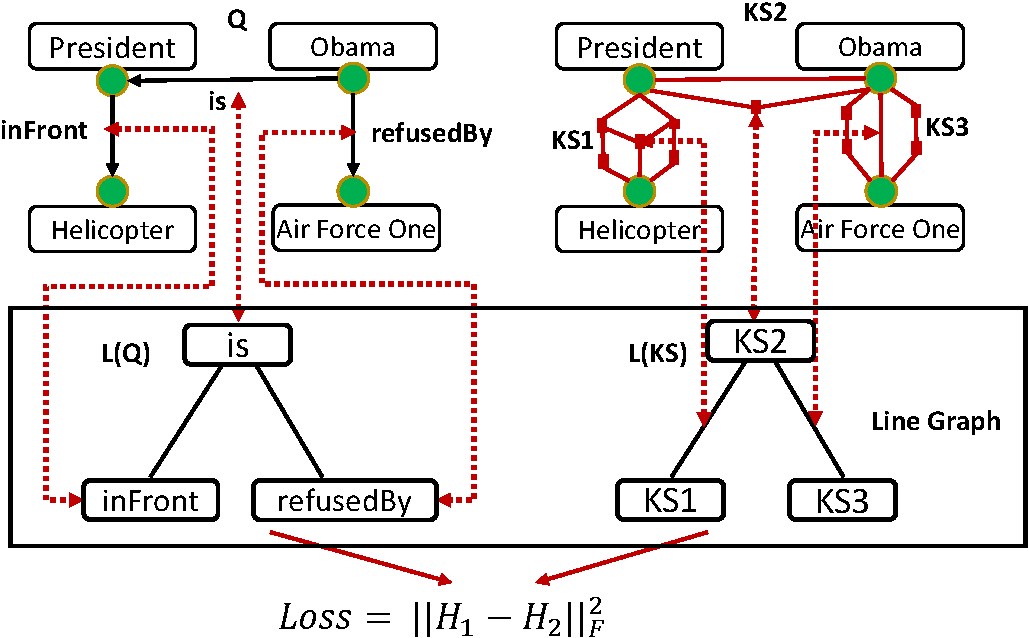
\includegraphics[width=0.5\textwidth]{submissions/logical-queries-uiuc/img/line-loss.pdf}
	\caption{Collective comparative reasoning workflow.}
	\label{collective-compare-workflow}
	\vspace{-1\baselineskip}
\end{figure}

To measure the importance of an element, we propose to use the influence function w.r.t. the distance between $L(Q)$ and $L(KS)$. We assume that a key element, if perturbed, would have a great effect on the distance
$\textrm{Loss} = || H_1 - H_2 ||_F^2$
%\hh{W1 and W2 have already been used in predicate-predicate similarity}
, where $H_1$ is the weighted adjacency matrix of $L(Q)$, and $H_2$ is the weighted adjacency matrix of $L(KS)$. We use the influence function $\frac{\partial \textrm{Loss}(H_1, H_2)}{\partial e}$, where $e$ represents an element of the knowledge segment graph and it could be a node, an edge, or a node attribute. Lemma~\ref{lm:collectiveinfluence} provides the details on how to compute such influence functions.

%If there are inconsistency in the query graph, after we correct such wrong node/edge attributes, it would significantly reduce the loss function. To this end,


\begin{lemma}\label{lm:collectiveinfluence}
Given the loss function $Loss = || H_1 - H_2 ||_F^2$. Let $n$, $k$ denote two different nodes in $L(Q)$,
and $KS_n$, $KS_k$ denote their corresponding knowledge segments.
Let $h_{e_{k,n}}$ denote the weight of edge between node $k$ and $n$,  and $h_{c_{k,n}}$ denote the weight of edge between $KS_k$ and $KS_n$. We have

\item [] (i) The influence of an edge $A_n(i,j)$ in knowledge segment $KS_n$ can be calculated as

$I(A_n(i,j)) = \sum_{k \in N(n)} -2(h_{e_{k,n}} - h_{c_{k,n}})\frac{\partial sim(KS_n, KS_k)}{\partial A_n(i,j)}$.

\item [] (ii) The influence of a node $i$ in knowledge segment $KS_n$ can be calculated as

$I(N_n(i)) = \sum_{k \in N(n)} -2(h_{e_{k,n}} - h_{c_{k,n}})\frac{\partial sim(KS_n, KS_k)}{\partial N_n(i)}$.

\item [] (iii) The influence of a node attribute $j$ in knowledge segment $KS_n$ can be calculated as

$I(N_n^j(i,i)) = \sum_{k \in N(n)} -2(h_{e_{k,n}} - h_{c_{k,n}})\frac{\partial sim(KS_n, KS_k)}{\partial N_n^j(i,i)}$.

\end{lemma}

\begin{proof}
We rewrite the loss function as
\setlength{\abovedisplayskip}{1pt}
\setlength{\belowdisplayskip}{1pt}
\begin{small}
\[
Loss = || H_1 - H_2 ||_F^2 = \sum_{i,j} (h_{e_{i,j}} - h_{c_{i,j}})^2
\vspace{-0.6\baselineskip}
\]
Take the derivative, together with Lemma 1, we have
\begin{equation}
\begin{aligned}
I(A_n(i,j)) &= \sum_{k \in N(n)} -2(h_{e_{k,n}} - h_{c_{k,n}})\frac{\partial sim(KS_n, KS_k)}{\partial A_n(i,j)} \\
\vspace{-0.6\baselineskip}
(N_n(i)) &= \sum_{k \in N(n)} -2(h_{e_{k,n}} - h_{c_{k,n}})\frac{\partial sim(KS_n, KS_k)}{\partial N_n(i)}  \\
I(N_n^l(i,i)) &= \sum_{k \in N(n)} -2(h_{e_{k,n}} - h_{c_{k,n}})\frac{\partial sim(KS_n, KS_k)}{\partial N_n^l(i,i)}
\end{aligned}
\end{equation}
\end{small}
which completes the proof.
\end{proof}


\textbf{Second}, after we find all the key elements, we check the consistency of the semantic matching subgraph according to these key elements. The steps are as follows.
For each pair of knowledge segments of the  semantic matching subgraph, if their key elements overlapping rate is greater than a threshold (60\%), we check the consistency of this pair. Suppose the corresponding triples are $<{\tt s_1}$, ${\tt p_1}$, ${\tt o_1}>$ and $<{\tt s_2}$, ${\tt p_2}$, ${\tt o_2}>$, respectively. We check if $<{\tt s_1}$, {\tt isTypeOf}, ${\tt s_2}>$ or $<{\tt s_2}$, {\tt isTypeOf}, ${\tt s_1}>$ is true. If both of them are false, we skip this pair of clues because it does not belong to C3 or C4. Otherwise, we check if $<{\tt o_1}$, {\tt isTypeOf}, ${\tt o_2}>$ or $<{\tt o_2}$, {\tt isTypeOf}, ${\tt o_1}>$ is true. If both of them are false, we say this query graph has collective inconsistency. When checking the truthfulness of triples (e.g., $<{\tt s_1}$, {\tt isTypeOf}, ${\tt s_2}>$,
$<{\tt s_2}$, {\tt isTypeOf}, ${\tt s_1}>$,
$<{\tt o_1}$, {\tt isTypeOf}, ${\tt o_2}>$ and $<{\tt o_2}$, {\tt isTypeOf}, ${\tt o_1}>$),
we use the same method (i.e., transferred information amount in Eq.~
\eqref{eq:transinfo}) as in pairwise comparative reasoning. 

\section{Experimental Results} \label{experiments}



In this section, we present the experimental evaluations. All the experiments are designed to answer the following two questions:

\begin{itemize}
	\item {\bf Q1. Effectiveness.} How effective are the proposed reasoning methods, including both pairwise and collective comparative reasoning methods?
	\item {\bf Q2. Efficiency.} How fast are the proposed methods? %The effectiveness of pair-wise comparative reasoning and collective comparative reasoning.
\end{itemize}


Two data graphs are used in the experiments: Yago ~\cite{yago} \footnote{It is publicly available at \url{https://www.mpi-inf.mpg.de/de/departments/databases-and-information-systems/research/yago-naga/yago/downloads}. We use the core version.} and Covid-19 \footnote{The dataset can be found at \url{http://blender.cs.illinois.edu/covid19/}. }.
Yago ~\cite{yago} is a widely used knowledge graph which contains 12,430,705 triples, 4,295,825 entities and 39 predicates.
The Covid-19 data graph contains three types of entities which are {\tt Gene}, {\tt Disease} and {\tt Chemical}.
In our experiments, we use a subset of the Covid-19 dataset which contains 55,434 core entities and 5,527,628 triples.
We compare our method with 4 baselines, including:

\begin{itemize}
    \item TransE ~\cite{transE} embeds both the entities and relations in the knowledge graph to a high dimension embedding space, and checks the consistency of a triple according to the embedding distance.
    \item Jaccard coefficient ~\cite{jaccard} is a link prediction algorithm which measures the truthfulness of the triple according to the number of common neighbor nodes of the head entity and tail entity.
    \item Knowledge Linker ~\cite{KL}, short for KL, extracts a path between the head entity and tail entity to decide whether the input triple is correct.
    \item KGMiner ~\cite{kgminer} extracts a subgraph between the head entity and tail entity to predict the truthfulness of the input clue.
    %\item KomPare ~\cite{kompare} leverages graph kernel to find important elements inside knowledge segments and make decision according to these important elements.
\end{itemize}

All the experiments are conducted on a moderate desktop with an Intel Core-i7 3.00GHz CPU and 64GB memory.
The source code could be found at \url{https://github.com/lihuiliullh/KompaRe}.
For TransE ~\cite{transE} in the experiments, we set the embedding dimension to 64 and use a margin of one and a learning rate of 0.01 for 1,200 epochs.










\subsection{Predicate-Predicate Similarity Efficacy}

\begin{figure}[ht]
\centering
	\begin{subfigure}[exports]{
		\centering
		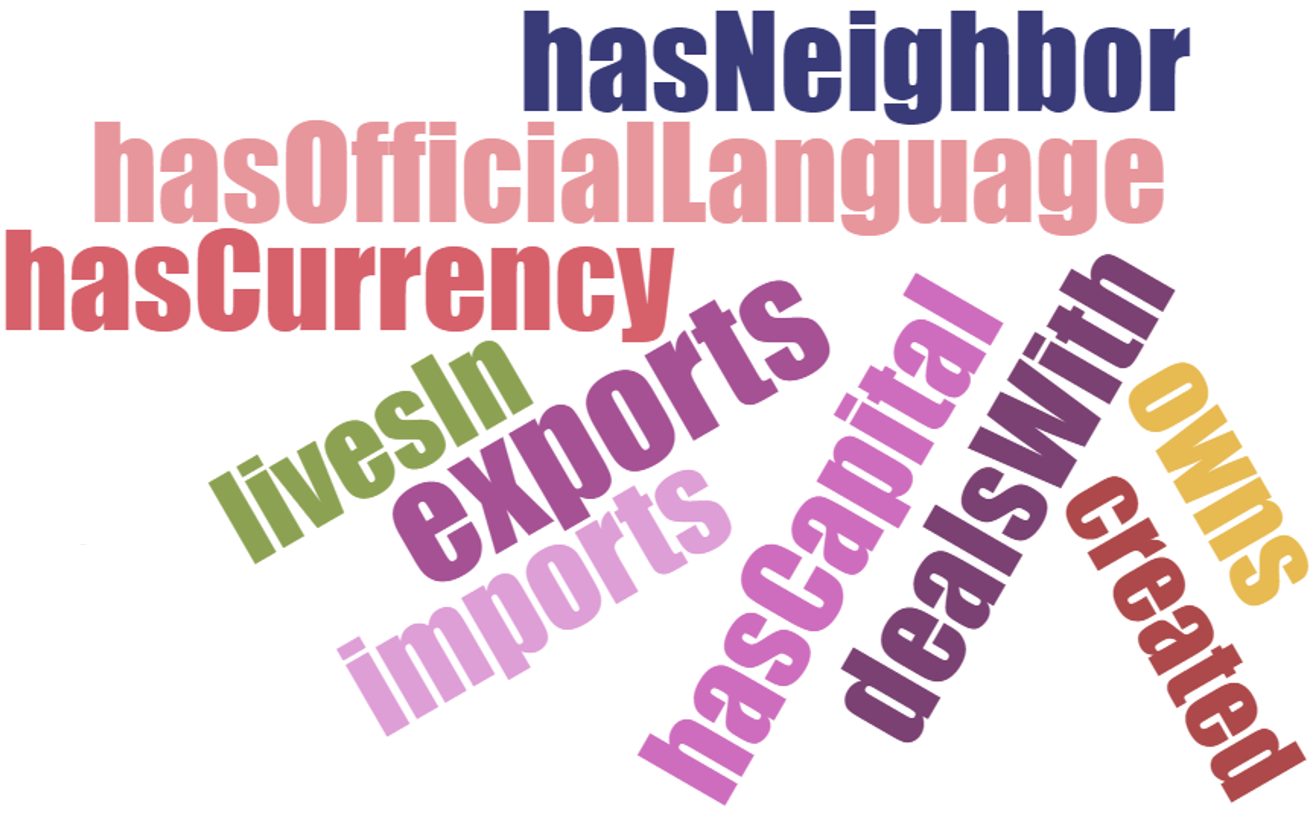
\includegraphics[width=0.35\textwidth]{submissions/logical-queries-uiuc/img/export.png}
		\label{subfig:dbqa}}
	\end{subfigure}
	\begin{subfigure}[livesIn]{
		\centering
		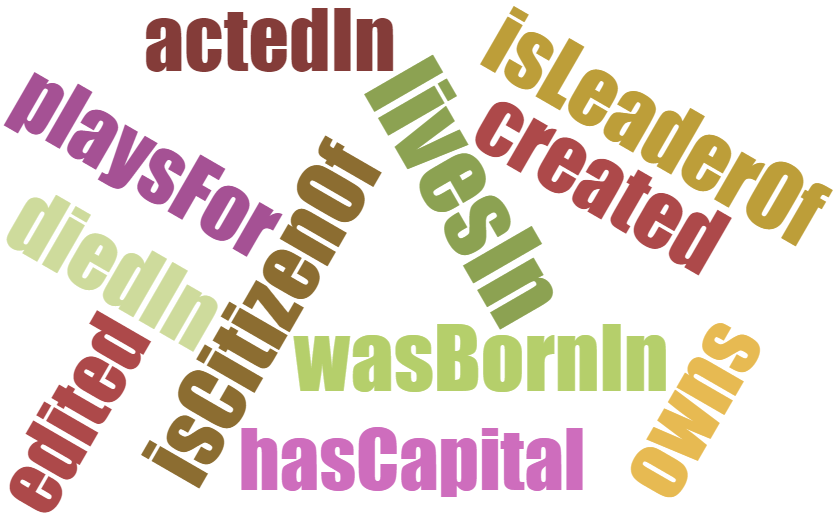
\includegraphics[width=0.35\textwidth]{submissions/logical-queries-uiuc/img/livesIn.png}
		\label{subfig:dbqa}}
	\end{subfigure}
%  \subfloat[exports]{
%	\begin{minipage}[c][0.5\width]{
%	   0.35\textwidth}
%	   \centering
%	   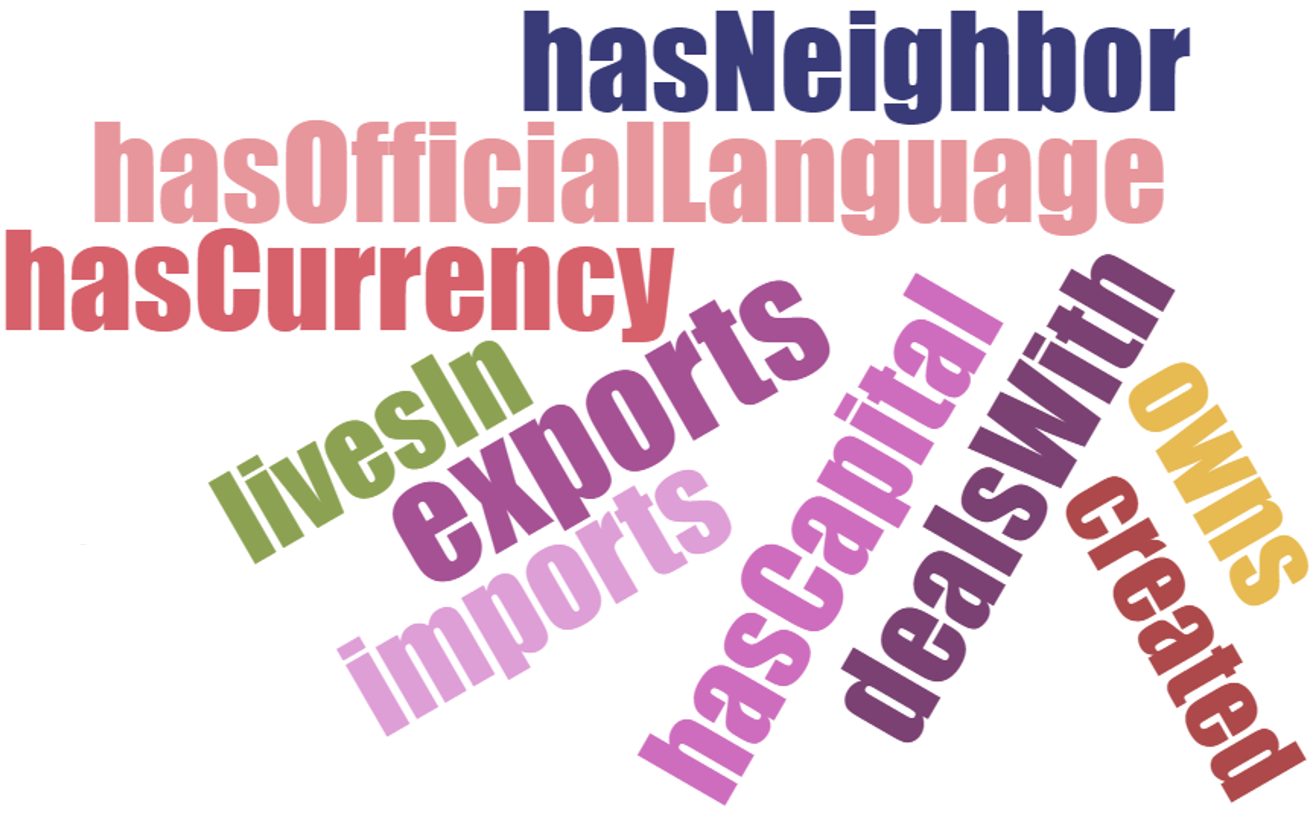
\includegraphics[width=1\textwidth]{submissions/logical-queries-uiuc/img/export.png}
%	\end{minipage}}
%%  \hfill 	
%\hspace{0.1\textwidth}
%  \subfloat[livesIn]{
%	\begin{minipage}[c][0.5\width]{
%	   0.35\textwidth}
%	   \centering
%	   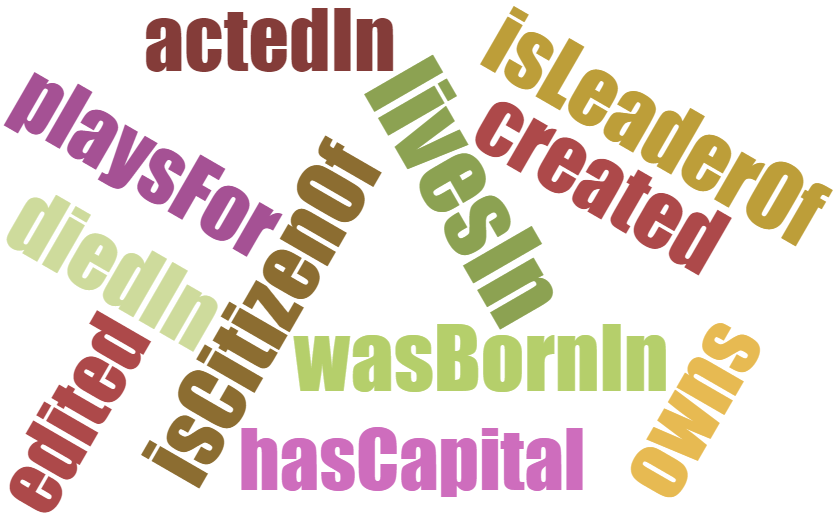
\includegraphics[width=1\textwidth]{submissions/logical-queries-uiuc/img/livesIn.png}
%	\end{minipage}}
\caption{Top-{\em 10} most similar predicates in Yago.}
\label{word-cloud}
\end{figure}

We evaluate the proposed predicate-predicate similarity. Figure ~\ref{word-cloud} presents two examples on Yago dataset. It shows the top-{\em 10} most similar predicates with {\tt exports} and {\tt livesIn}, respectively. The font size in Figure~\ref{word-cloud} is proportional to the predicate-predicate similarity value.
The top similar predicates w.r.t. {\tt exports} by our method include {\tt imports}, {\tt hasOfficialLanguage}, {\tt dealsWith}, all of which have a high similarity with {\tt exports}. They all provide specific semantic information about {\tt exports}.
Likewise, the top similar predicates w.r.t. {\tt livesIn} include {\tt wasBornIn}, {\tt isCitizenOf}, {\tt diedIn}, all of which are closely related to {\tt livesIn}. %They all talk about information related to some places or countries.
These results showcase that the proposed TF-IDF based method can effectively measure the similarity between different predicates.

Table ~\ref{appendix-pred-sim} shows the predicate similarity between {\tt isTypeOf} and other predicates. %We only list the predicates we used in this paper.
\begin{table}[!htbp]
    \centering
    \scriptsize
    \caption{Predicate similarity of {\tt isTypeOf} with others}
    \vspace{-1\baselineskip}
    \begin{tabular}{ |c|c|c|c|c|c|c|c| }
  \hline
  predicate & sim & predicate & sim & predicate & sim & predicate & sim \\
  \hline
 isCitizenOf &  0.840 &  isLeaderOf &  0.955 & isAffiliatedTo &  0.808 &  isPoliticianOf &  0.917 \\
 livesIn &  0.972 &  owns &  0.945 & exports &  0.706 &  dealsWith &  0.697\\
 hasCapital &  0.786 &  command &  0.216 & happenedIn &  0.767 &  participatedIn &  0.869\\
 worksAt &  0.752 &  isLocatedIn &  0.870 & & & &\\
  \hline
\end{tabular}
\label{appendix-pred-sim}
\end{table}


\vspace{-1.0\baselineskip}
\subsection{Pair-wise Comparative Reasoning}\label{exp-pair-section}

\begin{table*}
	\centering
	\caption{Accuracy of pair-wise comparative reasoning.
	}
	\scriptsize
	\vspace{-1\baselineskip}
	\setlength\tabcolsep{1.5pt}
	\begin{tabular}{|c|c|c|c|c|c|c|c|c|c|c|c|c|}
	\hline
	Dataset       & \makecell{\# of \\ queries}   & TransE & Jaccard  & KL  & KGMiner & Neural Network Based & Graph Kernel Based \\ \hline
	\makecell{Family members positive}   & 300  & 0.682 & 0.831 & 0.618 & {0.983} & \textbf{1.000} & 0.944 \\ \hline
	\makecell{Family members negative}   & 300  & 0.335 & 0.169 & \textbf{1.000} & \textbf{1.000} & 0.000 & 0.941 \\ \hline
    \makecell{Graduated college positive} & 300  & 0.686 & 0.335 & 0.502 & 0.769 &  \textbf{0.879} & {0.794} \\ \hline
    \makecell{Graduated college negative} & 300  & 0.626 & 0.993 & 0.947 & 0.901 & 0.367 & \textbf{0.994} \\ \hline
    \makecell{Live place positive}     & 300    & 0.567 & 0.415 & 0.489 & \textbf{0.834} & 0.086 & 0.762 \\ \hline
    \makecell{Live place negative}    & 300    & 0.802 & 0.585 & \textbf{0.907} & 0.900 & 0.732 & 0.888 \\ \hline
    \makecell{Birth place positive}    & 300    & 0.590 & 0.435 & 0.537 & 0.698 & 0.656 & \textbf{0.800} \\ \hline
    \makecell{Birth place negative}    & 300    & 0.845 & \textbf{1.000} & 0.973 & 0.927 & 0.719 & 0.927 \\ \hline
    \makecell{Work place positive}     & 300    & \textbf{0.751} & 0.319 & 0.445 & 0.698 & 0.700 & {0.720} \\ \hline
    \makecell{Work place negative}     & 300    & 0.624 & 0.994 & 0.942 & 0.927 & 0.803 & \textbf{0.995} \\ \hline
    $mean \pm std$  & - & 0.651 $\pm$ 0.424 & 0.608 $\pm$ 0.302 & 0.736 $\pm$ 0.221 & 0.864 $\pm$ 0.105 & 0.594 $\pm$ 0.333 & \textbf{0.877 $\pm$ 0.095}  \\ \hline
	\end{tabular}
\label{pair_dataset}
\end{table*}
Here, we evaluate the effectiveness of the proposed pair-wise comparative reasoning.
Ten query sets are used in the experiments.
For each positive query set, it contains a set of queries which describe the true claim, while for each negative query set, it contains a set of queries which describe the false claim. For example, in query set ``Birth Place", $<${\tt Alan Turing}, {\tt wasBornIn}, {\tt Maida Vale}$>$ and $<${\tt Alan Turing}, {\tt wasBornIn}, {\tt United Kingdom}$>$ is a positive query pair, while $<${\tt Alan Turing}, {\tt wasBornIn}, {\tt Maida Vale}$>$ and $<${\tt Alan Turing}, {\tt wasBornIn}, {\tt Canada}$>$ is an negative query pair.
The positive queries are generated by sampling some true claims in the knowledge graph. The negative queries are generated by substituting one subject of the positive queries.
The accuracy is defined as $\frac{N}{M}$ where $N$ is the number of queries correctly classified by pair-wise comparative reasoning and $M$ is the total number of queries.
When checking the consistency of a query pair $<{\tt s_1}, {\tt p_1}, {\tt o_1}>$ and $<{\tt s_2}, {\tt p_2}, {\tt o_2}>$,
because none of the baseline methods is designed for pair-wise comparative reasoning, we use them to check each triple in the pair, if any triple is classified as false, this query pair is treated as false. Otherwise, we further check the
truthness of $<{\tt o_1}, {\tt isTypeOf}, {\tt o_2}>$ and $<{\tt o_2}, {\tt isTypeOf}, {\tt o_1}>$,
if one of them is classified as consistency, this query pair is treated as consistency.
Table ~\ref{pair_dataset} gives the detailed results.


As we can see, Graph Kernel based method and KGMiner ~\cite{kgminer} have the highest accuracy most of the time. But Graph Kernel based method has the highest average accuracy and the lowest variance compared with other methods.

\subsection{Neural Network Based Pair-wise Comparative Reasoning}
We conduct more experiments in this section to test the effectiveness of Neural Network Based Pairwise comparative reasoning.
Six binary classifiers are used in the experiment. Table ~\ref{pair_dataset_bin_3} shows the details of each classifier and their performance on different query sets.
As we can see, different methods have different performances. Logistic Regression has the highest average accuracy and K-Nearest Neighbor has the highest average recall.


\begin{table}[!htbp]
\begin{adjustwidth}{-.5in}{-.5in}
        \begin{center}
    \centering
	\caption{Accuracy, recall and precision of neural network based pair-wise comparative reasoning
	}
	\scriptsize
	\vspace{-1\baselineskip}
	\setlength\tabcolsep{1.5pt}
	\begin{center}
	\begin{tabular}{|c|c|c|c|c|c|c|c|c|c|c|c|c|c|c|c|c|c|c|}
	\hline
	
 \diagbox{Model}{Dataset} & \multicolumn{3}{c|}{Family members} & \multicolumn{3}{c|}{Graduated college}& \multicolumn{3}{c|}{Live place}&\multicolumn{3}{c|}{Birth place}& \multicolumn{3}{c|}{Work place}& \multicolumn{3}{c|}{$mean \pm std$ }\\\hline

  measurements  & Acc & Prec & Recall & Acc & Prec & Recall &Acc & Prec & Recall &Acc & Prec & Recall &Acc & Prec & Recall &Acc & Prec & Recall\\
    \hline


% 	 &\makecell{family members}&\makecell{family members}&\makecell{family members} &\makecell{family members}&\makecell{family members} &\makecell{family members} \\ \hline
% 	 \multicolumn{1}{|c|}{messurements}  & Acc & Prec & Recall & Acc & Prec & Recall& Acc & Prec & Recall& Acc & Prec & Recall& Acc & Prec & Recall& Acc & Prec & Recall\\\hline
	\# of  queries &  \multicolumn{3}{c|}{506} & \multicolumn{3}{c|}{499} & \multicolumn{3}{c|}{560} & \multicolumn{3}{c|}{470} & \multicolumn{3}{c|}{540} & \multicolumn{3}{c|}{-} \\ \Xhline{1.5pt}
% 	Logistic Regression   &.682 & 0.831 & 0.618 & {0.983} \\ \hline
%     Support Vector Machines  & 0.686 & 0.335 & 0.502 & 0.769  \\ \hline
%     Decision Trees          & 0.567 & 0.415 & 0.489 &090\\ \hline
%     Random Forest      & 0.590 & 0.435 & 0.537 & 0.698  \\ \hline
%     Naive Bayes         & \textbf{0.751} & 0.319 & 0.445 & 0.698 \\ \hline
%     K-Nearest Neighbor      & \textbf{0.751} & 0.319 & 0.445 & 0.698 \\ \hline
Logistic Regression & 0.480 & 0.519 & 0.491 & 0.693 & 0.660 & 0.729 & 0.619 & 0.732 & 0.594 & 0.674 & 0.816 & 0.645 & 0.743 & 0.786 & 0.733 & \textbf{0.642}$\pm$\textbf{0.090} & 0.703$\pm$0.106 & 0.639$\pm$0.091 \\ \hline
SVM & 0.431 & 0.154 & 0.364 & 0.416 & 0.113 & 0.333 & 0.611 & 0.768 & 0.581 & 0.516 & 1.000 & 0.516 & 0.688 & 0.911 & 0.637 & 0.532$\pm$0.104 & 0.589$\pm$0.380 & 0.486$\pm$0.119 \\ \hline
Decision Trees & 0.422 & 0.519 & 0.443 & 0.713 & 0.623 & 0.786 & 0.619 & 0.696 & 0.600 & 0.611 & 0.694 & 0.607 & 0.716 & 0.750 & 0.712 & 0.616$\pm$0.107 & 0.656$\pm$\textbf{0.080} & 0.629$\pm$0.116 \\ \hline
Random Forest & 0.314 & 0.462 & 0.364 & 0.624 & 0.528 & 0.683 & 0.673 & 0.714 & 0.656 & 0.684 & 0.673 & 0.702 & 0.706 & 0.661 & 0.740 & 0.600$\pm$0.146 & 0.608$\pm$0.096 & 0.629$\pm$0.135 \\ \hline
Naive Bayes & 0.461 & 0.615 & 0.478 & 0.624 & 0.830 & 0.603 & 0.522 & 0.839 & 0.511 & 0.632 & 0.878 & 0.597 & 0.725 & 0.911 & 0.671 & 0.593$\pm$0.092 & \textbf{0.815}$\pm$0.104 & 0.572$\pm$\textbf{0.069} \\ \hline
K-Nearest Neighbor & 0.392 & 0.500 & 0.419 & 0.683 & 0.774 & 0.672 & 0.646 & 0.589 & 0.660 & 0.695 & 0.673 & 0.717 & 0.761 & 0.821 & 0.742 & 0.636$\pm$0.127 & 0.672$\pm$0.118 & \textbf{0.642}$\pm$0.115 \\ \hline
	\end{tabular}
\end{center}
\label{pair_dataset_bin_3}
\end{center}
    \end{adjustwidth}
\end{table}

Table ~\ref{pair_dataset_bin_Acc} shows performance of the neural network based method on each positive and negative query dataset. Based on the results in the table, we can conclude that the accuracy of the neural network based model is lower than that of other models, e.g., KGMiner and Graph Kernel Based method.

\begin{table}[!htbp]
	\centering
	\caption{Accuracy of neural network based pair-wise comparative reasoning
	}
	\scriptsize
	\vspace{-1\baselineskip}
	\setlength\tabcolsep{1.5pt}
	\begin{tabular}{|c|c|c|c|c|c|c|c|}
	\hline

\diagbox{Dataset}{Model} & \makecell{\# of \\ queries}   & Logistic Regression & Support Vector Machines & Decision Trees  & Random Forest & Naive Bayes & K-Nearest Neighbor\\ \hline
Family members positive & 258& 0.519 & 0.577 & 0.481 & 0.481 & 0.615 & 0.500\\ \hline
Family members negative & 248& 0.440 & 0.420 & 0.340 & 0.260 & 0.300 & 0.280\\ \hline
Graduated college positive & 261& 0.660 & 0.868 & 0.623 & 0.547 & \textbf{0.830} & 0.774\\ \hline
Graduated college negative & 238& 0.729 & 0.208 & \textbf{0.812} & \textbf{0.708} & 0.396 & 0.583\\ \hline
Live place positive & 277& 0.732 &\textbf{1.000} & 0.643 & 0.679 & 0.839 & 0.589\\ \hline
Live place negative & 283& 0.509 & 0.632 & 0.526 & 0.632 & 0.211 & 0.702\\ \hline
Birth place positive & 244& \textbf{0.816} & \textbf{1.000} & 0.653 & 0.653 & 0.878 & 0.673\\ \hline
Birth place negative & 226& 0.522 & 0.000 & 0.522 & 0.674 & 0.370 & 0.717\\ \hline
Work place positive & 277& 0.786 & 0.946 & 0.696 & 0.679 & 0.911 & \textbf{0.821}\\ \hline
Work place negative & 263& 0.698 & \textbf{1.000} & 0.660 & 0.755 & 0.528 & 0.698\\ \hline
$mean \pm std$ & - & 0.641 $\pm$ 0.126 & \textbf{0.665} $\pm$ 0.343 & 0.596 $\pm$ \textbf{0.125} & 0.607 $\pm$  0.138 & 0.588 $\pm$ 0.250 & 0.634 $\pm$ 0.148 \\ \hline

	\end{tabular}
\label{pair_dataset_bin_Acc}
\end{table}


\hide{
\begin{figure}[]
	\centering
	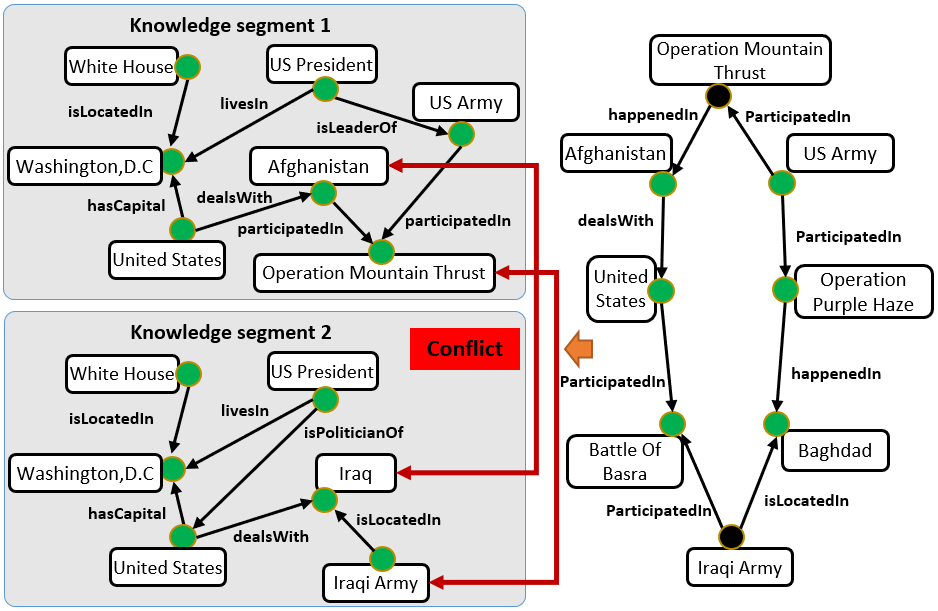
\includegraphics[width=0.47\textwidth]{img/iraq_operation.png}
	\caption{Pair-wise comparative reasoning results.}
	\label{iraq_inconsistency-example}
	\vspace{-1\baselineskip}
\end{figure}

\begin{figure}[]
	\centering
	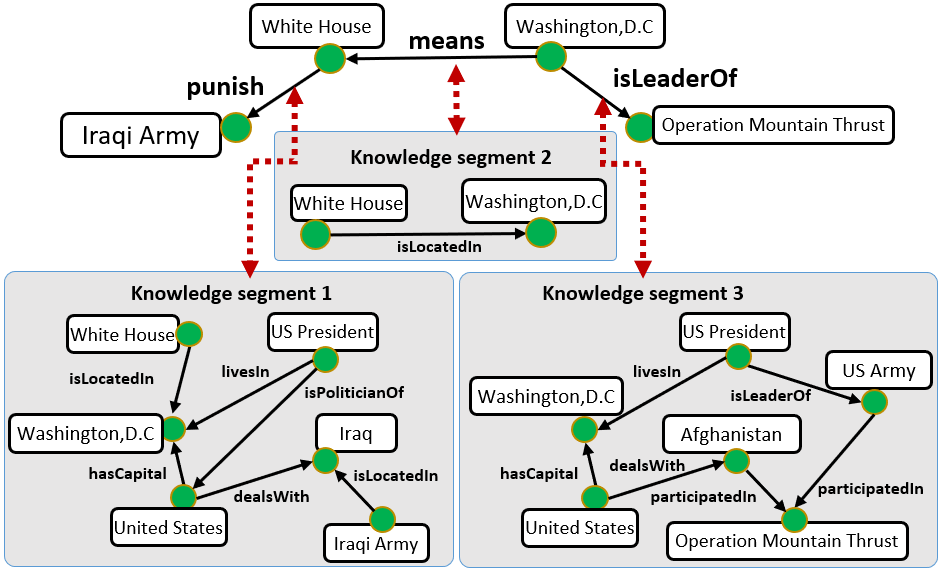
\includegraphics[width=0.47\textwidth]{img/iraq_collect.png}
	\caption{Collective comparative reasoning results.}
	\label{iraq_exp-coll}
	\vspace{-1\baselineskip}
\end{figure}
}



\vspace{-0.6\baselineskip}
\subsection{Collective Comparative Reasoning}\label{exp-coll-section}
\hide{
Here, we evaluate the effectiveness of the proposed collective comparative reasoning.
We test a query graph with three edges, including <{\tt White House}, {\tt punish}, {\tt Iraqi Army}>, <{\tt Washington,D.C}, {\tt means}, {\tt White House}> and <{\tt Washington,D.C}, {\tt participatedIn}, {\tt Operation Mountain Thrust}>.
Figure ~\ref{iraq_exp-coll} shows the query graph and the corresponding semantic matching subgraph.
As we can see, if we use the pair-wise comparative reasoning method to check each pair of them, all of them are true. %\footnote{For the query pair: <{\tt White House}, {\tt punish}, {\tt Iraqi Army}>, <{\tt Washington,D.C}, {\tt isLeaderOf}, {\tt Operation Mountain Thrust}>. Because these two clues have different subjects, so we won't check their inconsistency.}
However, if we use the collective comparative reasoning method, we could detect the inconsistency in the query graph as follows.

Table~\ref{iraq_coll-node-attr} and Table~\ref{iraq_coll-edge1} in Appendix show the node attribute influence, the node influence, and the edge influence of these three knowledge segments, respectively.
If we check each pair of clues in the query graph, we find that the key elements overlapping rate between $KS_1$ and $KS_3$ is more than 60\%. This is because the overlapping rates  are $66.6\%$ for node attribute influence, $100\%$ for node influence and $66.6\%$ for edge influence, which give the average overlapping rate $\frac{\frac{2}{3} + 1 + \frac{2}{3}}{3} = \frac{7}{9} > 60\%$.

Based on this, we future check <{\tt Washington,D.C}, {\tt isTypeOf}, {\tt White House}> or <{\tt White House}, {\tt isTypeOf}, {\tt Washington,D.C}>.
Our TF-IDF based predicate-predicate similarity between "{\tt isTypeOf}" and "{\tt isLocatedIn}" is 0.870. Thus, we have \textrm{infTrans}({\tt Washington,D.C}, {\tt White House}) $= 0.870 > 0.700$. This means that these two knowledge segments have the same subject. Finally, we check  <{\tt Operation Mountain Thrust}, {\tt isTypeOf}, {\tt Iraqi Army}> or <{\tt Iraqi Army}, {\tt isTypeOf}, {\tt Operation Mountain Thrust}>. According to the results in the previous subsection, we have that {\tt Iraqi Army} and {\tt Operation Mountain Thrust} are two different things. Therefore, we conclude that this query graph is inconsistent.

}


\begin{table}[!htbp]
	\centering
	\caption{Accuracy of collective comparative reasoning.}
	\fontsize{9}{9}\selectfont
	\setlength\tabcolsep{0.8pt}
	\begin{tabular}{|c|c|c|c|c|c|c|c|c|c|c|c|c|}
	\hline
	Dataset       & \makecell{\# of \\ queries}   & TransE & Jaccard  & KL  & KGMiner & Kompare \\ \hline
    Birth place positive   & 300     & 0.542 & 0.418 & 0.389 & 0.678 & \textbf{0.795} \\ \hline
    Birth place negative   & 300     & 0.465 & \textbf{0.996} & 0.968 & 0.970 & 0.829 \\ \hline
    Live place positive    & 300     & 0.448 & 0.451 & 0.465 & 0.635 & \textbf{0.989} \\ \hline
    Live place negative    & 300     & 0.558 & \textbf{1.000} & 0.860 & 0.924 & 0.743 \\ \hline
    Graduated college positive & 300  & 0.488 & 0.269 & 0.335 & 0.585 & \textbf{0.963} \\ \hline
    Graduated college negative & 300  & 0.545 & \textbf{0.996} & 0.928 & 0.907 & 0.829 \\ \hline

    $mean \pm std$ & - & 0.508 $\pm$ \textbf{0.045}  & 0.688 $\pm$ 0.313 & 0.658 $\pm$ 0.265 & 0.783 $\pm$ 0.155 & \textbf{0.858} $\pm$ 0.089  \\ \hline
    %Variance & - & \textbf{0.002} & 0.098 & 0.070 & 0.024 & 0.008  \\ \hline
	\end{tabular}
\label{coll_dataset}
\end{table}


We test collective comparative reasoning method on Yago dataset, using 6 query sets .
Different from the queries of pair-wise comparative reasoning which only contain two edges, each query of collective comparative reasoning contains 3 edges.
For example, in query set ``live Place", $<${\tt Barack Obama}, {\tt livesIn}, {\tt Washington,D.C.}$>$, $<${\tt Barack Obama}, {\tt is}, {\tt United States Senate Barack Obama}$>$ and $<${\tt United States Senate Barack Obama}, {\tt livesIn}, {\tt United States}$>$ is a positive query triad, while $<${\tt Barack Obama}, {\tt livesIn}, {\tt Washington,D.C.}$>$, $<${\tt Barack Obama}, {\tt is}, {\tt United States Senate Barack Obama}$>$ and $<${\tt United States Senate Barack Obama}, {\tt livesIn}, {\tt Canada}$>$ is an negative query triad.
The definition of the accuracy is the same as the previous section.
Following the setting of pair-wise reasoning, when checking the consistency of the query graph $<{\tt s_1}, {\tt p_1}, {\tt o_1}>$, $<{\tt s_1}, {\tt is}, {\tt s_2}>$ and $<{\tt s_2}, {\tt p_2}, {\tt o_2}>$,
we use baseline methods to check the truthness of this query triad, if any edge is classified as false, this query triad is treated as false. Otherwise,
we further check the truthness of $<{\tt o_1}, {\tt isTypeOf}, {\tt o_2}>$ and $<{\tt o_2}, {\tt isTypeOf}, {\tt o_1}>$,
if one of them is classified as true , this query pair is treated as consistency.
%\hh{double check: here you say 'if one of them is consistent/true' and in the covid19 paragraph (below), you say 'if any edge is ... false' which is which?}
Table ~\ref{coll_dataset} gives the detailed results.
As we can see, Jaccard ~\cite{jaccard} prefers to classify all queries as inconsistency and has the largest variance.
TransE ~\cite{transE} has the lowest variance, but its average accuracy is very low. \gchecker\ has the highest accuracy most of the time. It also has the highest average accuracy, and the second lowest variance.

%\subsection{Covid-19 Results}

\begin{table}[h]
	\centering
	\caption{Accuracy of collective comparative reasoning for Covid-19.}
	\fontsize{8}{9}\selectfont
	\setlength\tabcolsep{1.5pt}
	\begin{tabular}{|c|c|c|c|c|c|c|c|c|c|c|c|c|}
	\hline
	Dataset    & \# of queries      & TransE & Jaccard  & KL  & KGMiner & Kompare \\ \hline
    Positive    & 36    & 0.667 & 0.611 & \textbf{1.000} & 0.694 & \textbf{1.000} \\ \hline
    Negative    & 36    & 0.528 & 0.361 & 0.722 & 0.553 & \textbf{0.863} \\ \hline
    Average accuracy &  - & 0.598 $\pm$ 0.071  & 0.486 $\pm$ 0.126 & 0.861 $\pm$ 0.138 & 0.623 $\pm$ 0.071 & \textbf{0.932 $\pm$ 0.063}  \\ \hline
    %Variance & - & 0.005 & 0.016 & 0.019 & 0.005 & \textbf{0.004} \\ \hline
	\end{tabular}
\label{covid_coll}
\end{table}

We further provide experimental results on Covid-19 dataset.
We use queries which contain connections between drugs and genes/chemicals related to covid-19.\footnote{The query graphs can be found at \url{http://blender.cs.illinois.edu/covid19/visualization.html}.}
Among all these queries, we use queries which contain less than 8 nodes, and treat them as positive queries.
For each of the positive queries, we randomly select one node inside the query and substitute it with a randomly selected entity in the data graph, and treat the new query as the negative query.
%Following the setting of collective comparative reasoning,
For all the baseline methods, we use them to check all the edges inside the query, if any edge is classified as false, the whole query is treated as false.
Table ~\ref{covid_coll} shows the accuracy of different methods.
As we can see, \gchecker\ has the highest accuracy on both the positive and negative datasets, it also has the highest average accuracy and the lowest variance compared with other baseline methods.


\subsection{Efficiency Results}

%\hh{we need some efficiency results, e.g., runtime for ks extraction w.r.t. the kg size; runtime for comparative reasoning  w.r.t. the kg size; }
The runtime of knowledge segment extraction depends on the size of the underlying knowledge graphs. Among the two types of knowledge segments (edge-specific knowledge segment and subgraph-specific knowledge segment), subgraph-specific knowledge segment is most time-consuming. Figure ~\ref{fig:runtime}(a) shows that its runtime scales sub-linearly w.r.t. the number of nodes in the knowledge graph. Different lines show the runtime w.r.t. different query graph size.
Figure ~\ref{fig:runtime}(b) shows the runtime of comparative reasoning, where `Pair-wise' refers to the pairwise comparative reasoning, and the remaining bars are for collective comparative reasoning with $3$, $4$ and $5$ edges in the query graphs respectively. Note that the runtime of comparative reasoning only depends on the size of the the corresponding knowledge segments which typically have a few or a few tens of nodes. In other words, the runtime of comparative reasoning is {\em independent} of the knowledge graph size.


%%%%%+++++++++++++++++++++++++++++++++++
\begin{figure}\label{fig:runtime}
\vspace{-0.8\baselineskip}
\centering
%\hide{
%%%%% hspace is used to control the row and columns
%\subfloat[][Node-specific Knowledge Segment Extraction Runtime]{%
%\label{node-runtime}%
%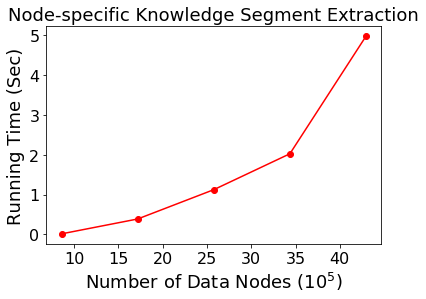
\includegraphics[height=1.7in]{img/node-specific-runtime.png}}%
%\hspace{50pt}%
%\subfloat[][Edge-specific Knowledge Segment Extraction Runtime]{%
%\label{edge-runtime}%
%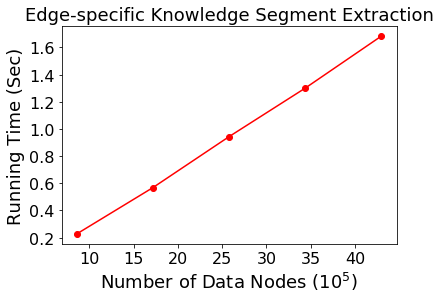
\includegraphics[height=1.7in]{img/edge-specific-runtime.png}}%
%}
%
%%\hspace{1pt}%
%\subfloat[h][Subgraph-specific KS extraction]{%
%\label{semantic-runtime-data}%
%\includegraphics[height=2in]{img/semantic-subgraph-data-time.png}}%
%%\hspace{50pt}%
%\subfloat[][Comparative reasoning]{%
%\label{comp-time}%
%\includegraphics[height=2in]{img/comparative-reasoning-runtime.png}}% \\
%%\hspace{1pt}%
	\begin{subfigure}[Subgraph-specific KS extraction]{
		\centering
		\includegraphics[width=0.45\textwidth]{submissions/logical-queries-uiuc/img/semantic-subgraph-data-time.png}
		\label{subfig:dbqa}}
	\end{subfigure}
	\begin{subfigure}[Comparative reasoning]{
		\centering
		\includegraphics[width=0.45\textwidth]{submissions/logical-queries-uiuc/img/comparative-reasoning-runtime.png}
		\label{subfig:dbqa}}
	\end{subfigure}
% \vspace{-1\baselineskip}
\caption[A set of four subfigures.]{
Runtime of \gchecker\
}
\label{precision-4}%
\label{fig:runtime}
\end{figure}
%%%%%+++++++++++++++++++++++++++++++++++





\section{Related Work}\label{related-work}


\bx{TODO: extend the related work}
{\bf A - Knowledge Graph Search.} Many efforts have been made for searching and browsing large knowledge graphs. 
Wang et al. ~\cite{Wang2015QUT} proposed a Bayesian probability model combined with random walks to find the most similar concepts for a given query entity.
Wu et al. ~\cite{YinghuiWu} discovered that the background knowledge graph can be described by many small-sized patterns. 
They developed an effective mining algorithm to summarize the large knowledge graph according to small-sized patterns.
Yang et al. ~\cite{Yang2014vldb} found that due to the lack of insight about the background knowledge graph, it is often hard for a user to precisely formulate a query. They developed a user-friendly knowledge graph search engine to support query formation and transformation. 
Jayaram et al. ~\cite{GQBE} proposed a knowledge graph query system called {\em GQBE}. Different from other graph query systems, {\em GQBE} focuses on entity tuple query which consists of a list of entity tuples.
Zhang et al. ~\cite{tongtao2018Gaia} developed a comprehensive multi-modality knowledge extraction and hypothesis generation system which supports three types of queries, including (1) class-based queries %which aim to find all instances of a known class in the knowledge graph; (e.g. find all "politician") 
(2) zero-hop queries %which aim to find all instances of an entity; (e.g. find all entities with name "Barack Obama") 
and (3) graph-queries. % which aim to find a graph. 

\noindent {\bf B - Fact Checking on Knowledge Graph. } In 2015, GL Ciampaglia et al. \cite{ciampaglia2015computational} show that the complexities of human fact checking can be approximated quite well by finding the shortest path between concept nodes under properly defined semantic proximity metrics on knowledge graphs. The authors evaluate tens of thousands of claims on knowledge graphs extracted from Wikipedia. Many research works follow this direction with different techniques. Baoxu et al. \cite{shi2016discriminative} model the fact checking problem as a link-prediction task in a knowledge graph, and present a discriminative path-based method for fact checking in knowledge graphs. Shiralkar et al. \cite{shiralkar2017finding} adopts k-shortest paths approach to construct a knowledge stream (KS) between two entities as the background knowledge for fact checking. Lin et al. \cite{lin2018fact} introduce ontological patterns in fact checking for semantic and topological constraints. These constraints are represented as subgraph patterns which are used for query in the knowledge graph. In order to obtain the ground truth of contextualized claim, Tchechmedjiev et al. release a large, up-to-date and queryable corpus of structured information about claims and related metadata for fact checking research, named ClaimsKG \cite{tchechmedjiev2019claimskg}. 


\noindent {\bf C - Knowledge Graph Reasoning.} Generally speaking, there are two types of knowledge graph reasoning methods, including (1) embedding based approaches and (2) multi-hop approaches. For the former, 
the main idea is to learn a low dimensional vector for each entity and predicate in the embedding space, and use these embedding vectors as the input of the reasoning tasks (e.g.,~\cite{transE}, ~\cite{rotatE}, ~\cite{entity-predicate}, ~\cite{pprop}).
For the latter, %\hh{1-2 sentenses on its key ideas and cite William cohen's random walk based method. William Wang's meta-reasoning method, etc.}
the main idea is to learn missing rules from a set of relational paths sampled from the knowledge graph (e.g.,~\cite{williamCohen}, ~\cite{willianWang}, ~\cite{das-etal-2017-chains}). Many effective reasoning methods have been developed for predicting the missing relation (i.e., link prediction) or the missing entity (i.e., entity prediction). 
In link prediction, given the `subject' and the `object' of {\em a triple}, it predicts the existence and/or the type of relation. 
For example,
{\em TransE}~\cite{transE} learns the low dimensional embedding of both entities and predicates in the knowledge graph; %. The relationship between two entities can be predicated by the translation between the embeddings of entities.
{\em TransR}~\cite{Lin2015TransR} learns the embedding of entities and predicates in two separate spaces. 
The learned embedding (either by {\em TransE} or {\em TransR}) can be used for both link predication and entity predication. 
%In ~\cite{SimplE}, \lliu{xxxxxxxxxx}. 
In entity prediction, given the `subject' and the `predicate' of {\em a triple}, it predicts the missing `object'. For example, 
%\hh{a few representative work, 1-2 sentences for each of them} 
{\em GQEs}~\cite{entity-predicate} embeds the graph nodes in a low dimensional space, and treats the logical operators as learned geometric operations.


In recent years, knowledge graph reasoning has demonstrated strong potential for computational fact checking. Given {\em a claim} in the form of a triple of the knowledge graph, it reasons whether the claim is authentic or falsified. For example, 
in ~\cite{Shiralkar2017}, the authors focused on checking the truthfulness of a given triple/claim, by first transforming the knowledge graph into a weighted directed graph, and then extracting a so-called knowledge stream based on maximum flow algorithm. %First, they transformed the knowledge graph into a line graph to model the co-occurrence of different predicates, and they used a TF-IDF method to calculate the similarity between different predicates. Then, they transferred the knowledge graph into a directed weighted graph and used a minimum cost maximum flow algorithm to find the knowledge stream between the give subject and object. If the truth score of the knowledge stream is too low, they thought that the query is false.
It is worth mentioning that the extracted knowledge stream can be viewed as an edge-specific knowledge segment in \gchecker. 
In ~\cite{Shi2016dpp}, an alternative method was developed to detect fake claims by learning the discriminative paths of specific predicates. Different from \cite{Shiralkar2017}, this is a supervised reasoning method since 
it requires different training datasets for different predicates. 
If the predicate in the claim does not exist in the training data, which is likely to be the case for detecting falsified claims in emerging news, the algorithm becomes inapplicable.
 As mentioned before, these methods belong to point-wise reasoning. Therefore, %Thus, although being effective in detecting a single falsified claim, 
 they might fall short in detecting the semantic inconsistency between multiple claims which can be solved by knowledge graph comparative reasoning.

%However, all the above methods focus on fact checking for a single claim, link predication or entity predication , and thus is incapable of detecting the semantic inconsistencies between different claims.


\hide{

\begin{table*}[]
	\centering
	\caption{Summary of Existing KG Search and Comparative Reasoning Systems}
	\vspace{-0.5\baselineskip}
	\resizebox{\textwidth}{!}{
	\begin{tabular}{|c|c|c|c|}
		\hline
		Name & Input                                              & Output         &       KG Systems    \\ \hline
		\tt{F1} & A single query node                                & Top-{\em k} Entities  & ~\cite{Tong2006rdwalk} ~\cite{Lin2015TransR} ~\cite{Mikolov2013DRW} \\ \hline
		\tt{F1'} & A single query node                             & A subgraph with most relevant entities and edges w.r.t the query node & None \\ \hline
		\tt{F2} & A Single query edge                                & Knowledge segment & ~\cite{Shiralkar2017} ~\cite{Shi2016dpp} ~\cite{lei2018} \\ \hline
		\tt{F3} & Two or more query edges                        & commonality and inconsistency & None \\ \hline
		\tt{F4} & A query graph                               & A matching subgraph  & ~\cite{Su2015KDD} ~\cite{lei2018} ~\cite{Zou2011GAS} ~\cite{Yahya2016RQE} \\ \hline
		\tt{F4'} & A query graph                               & A semantic matching subgraph/Knowledge Segment  & None \\ \hline
		%~\cite{Faloutsos2004} ~\cite{Tong2006CSP} ~\cite{Su2015KDD} ~\cite{Tong2007FBP} ~\cite{lei2018} \\ \hline
		%multiple query nodes                               & \thead{Connection Pathways \\ for Marked Nodes} & ~\cite{Koren2006MEP} ~\cite{Tong2006CSP}  \\ \hline
		\tt{F5} & Multiple query nodes               & Grouping and connection pathways & None \\ \hline
		\tt{F6} & A single node/edge and multiple KG               & Commonality and differences in different KGs & None \\ \hline
		\end{tabular}
	}
\label{table:existing:kgsys}
\vspace{-0.8\baselineskip}
\end{table*}
}


%\hh{have u checked this tutorial? \url{https://sites.cs.ucsb.edu/~william/papers/Part3_KB_Reasoning.pdf}? seems that we have already consider these tasks, link prediction, entitiy prediction, fact checking. just make sure we do not miss important aspect of kg reason from existing work}
%\lliu{Hi professor, I have checked this tutorial before. I will add more work about kg reason here.}
%\hh{check this paper~\cite{Leman2013SIAM} -- some components of their system might be related to KG search and reasoning}

%In ~\cite{qi2018ICDE}, the authors proposed a graph summarization framework to facilitate knowledge graph search. They first summarize the knowledge graph into a concreate graph according to some frequent graph pattern, then they find the (approximate) answers according to the query. 
%\hh{a little bit more details, e.g., what is the main functions (in input/output format)?}
%In ~\cite{Su2015KDD}, they used the feedback information to enhance the knowledge graph query performance.
%In ~\cite{slq2014vldb}, they proposed a system SLQ.


%\vspace{-0.9\baselineskip}
\section{Conclusions}\label{conclusion}




In this paper, we present the problem definition and algorithms for knowledge graph comparative reasoning. 
Comparative reasoning aims to complement and expand the existing point-wise reasoning over knowledge graphs by inferring commonalities and inconsistencies of multiple pieces of clues.
We propose several methods to tackle comparative reasoning.
At the heart of the proposed methods are a suite of core algorithms, including predicate-predicate similarity and semantic subgraph matching for knowledge segment extraction; neural network and influence function, commonality rate, transferred information amount for both pairwise reasoning and collective reasoning. 
The experimental results demonstrate that the proposed methods (1) can effectively detect semantic inconsistency, and (2) scales near linearly with respect to the knowledge graph size. 



%
\section{Timeline}

\begin{itemize}
    \item Revise paper. Covid19 experiments. Dec 18 - Dec 25.
    \item Revise paper. Dec 25 - Dec 31.
\end{itemize}






%\bibliographystyle{plain}
%\bibliography{submissions/logical-queries-uiuc/008reference}

%%
%% If your work has an appendix, this is the place to put it.

\begin{thebibliography}{10}

\bibitem{transE}
B.~Antoine, U.~Nicolas, G.~Alberto, W~Jason, and Y.~Oksana.
\newblock Translating embeddings for modeling multi-relational data.
\newblock In {\em NIPS '13}, NIPS '13, pages 2787--2795.

\bibitem{KL}
Giovanni~Luca Ciampaglia, Prashant Shiralkar, and Rocha.
\newblock Computational fact checking from knowledge networks.
\newblock 2015.

\bibitem{ciampaglia2015computational}
Giovanni~Luca Ciampaglia, Prashant Shiralkar, Luis~M Rocha, Johan Bollen,
  Filippo Menczer, and Alessandro Flammini.
\newblock Computational fact checking from knowledge networks.
\newblock {\em PloS one}, 10(6):e0128193, 2015.

\bibitem{Cui2019SAMES}
Limeng Cui, Suhang Wang, and Dongwon Lee.
\newblock Same : Sentiment-aware multi-modal embedding for detecting fake news.
\newblock 2019.

\bibitem{bert}
Jacob Devlin, Ming-Wei Chang, Kenton Lee, and Kristina Toutanova.
\newblock Bert: Pre-training of deep bidirectional transformers for language
  understanding, 2018.

\bibitem{sysvester}
Boxin Du, Lihui Liu, and Hanghang Tong.
\newblock Sylvester tensor equation for multi-way association.
\newblock In {\em Proceedings of the 27th ACM SIGKDD Conference on Knowledge
  Discovery and Data Mining}, KDD '21, page 311–321, New York, NY, USA, 2021.
  Association for Computing Machinery.

\bibitem{Faloutsos2004}
C.~Faloutsos, K.~McCurley, and A.~Tomkins.
\newblock Fast discovery of connection subgraphs.
\newblock In {\em KDD '04}, pages 118--127, New York, NY, USA, 2004. ACM.

\bibitem{Freitas}
S.~{Freitas}, N.~{Cao}, Y.~{Xia}, D.~H.~P. {Chau}, and H.~{Tong}.
\newblock Local partition in rich graphs.
\newblock BigData '19, pages 1001--1008, Dec 2018.

\bibitem{knowledge-path}
C.~Giovanni, S.~Prashant, R.~Luis, B.~Johan, M.~Filippo, and F.~Alessandro.
\newblock Computational fact checking from knowledge networks.
\newblock {\em PloS one}, 10, 01 2015.

\bibitem{GQBE}
N.~{Jayaram}, A.~{Khan}, C.~{Li}, X.~{Yan}, and R.~{Elmasri}.
\newblock Querying knowledge graphs by example entity tuples.
\newblock 27(10):2797--2811, Oct 2015.

\bibitem{Koren2006MEP}
Y.~Koren, S.~North, and C.~Volinsky.
\newblock Measuring and extracting proximity in networks.
\newblock KDD '06, pages 245--255, New York, NY, USA, 2006. ACM.

\bibitem{entity-predicate}
H.~William L., B.~Payal, Z.~Marinka, J.~Dan, and L.~Jure.
\newblock Embedding logical queries on knowledge graphs.
\newblock NIPS’18, page 2030–2041, Red Hook, NY, USA, 2018.

\bibitem{williamCohen}
Ni~L, Tom M, and William~W. C.
\newblock Random walk inference and learning in a large scale knowledge base.
\newblock EMNLP ’11, USA, 2011.

\bibitem{jaccard}
David Liben-Nowell and Jon Kleinberg.
\newblock The link prediction problem for social networks.
\newblock CIKM '03.

\bibitem{lin2018fact}
Peng Lin, Qi~Song, and Yinghui Wu.
\newblock Fact checking in knowledge graphs with ontological subgraph patterns.
\newblock {\em Data Science and Engineering}, 3(4):341--358, 2018.

\bibitem{Lin2015TransR}
Y.~Lin, Z.~Liu, M.~Sun, Y.~Liu, and X.~Zhu.
\newblock Learning entity and relation embeddings for knowledge graph
  completion.
\newblock AAAI'15. AAAI Press, 2015.

\bibitem{lihui}
L.~{Liu}, B.~{Du}, and H.~{Tong}.
\newblock Gfinder: Approximate attributed subgraph matching.
\newblock BigData '19, Dec 2019.

\bibitem{kompare}
Lihui Liu, Boxin Du, Yi~Ren Fung, Heng Ji, Jiejun Xu, and Hanghang Tong.
\newblock Kompare: A knowledge graph comparative reasoning system.
\newblock In {\em Proceedings of the 27th ACM SIGKDD Conference on Knowledge
  Discovery and Data Mining}, KDD '21, page 3308–3318, New York, NY, USA,
  2021. Association for Computing Machinery.

\bibitem{prototype_liu}
Lihui Liu, Boxin Du, Heng Ji, and Hanghang Tong.
\newblock A knowledge graph reasoning prototype.
\newblock {\em NeurIPS (demo track)}, 2020.

\bibitem{binet}
Lihui Liu, Boxin Du, Jiejun Xu, Yinglong Xia, and Hanghang Tong.
\newblock Joint knowledge graph completion and question answering.
\newblock In {\em Proceedings of the 28th ACM SIGKDD Conference on Knowledge
  Discovery and Data Mining}, KDD '22, page 1098–1108, New York, NY, USA,
  2022. Association for Computing Machinery.

\bibitem{multimodal}
Kai Nakamura, Sharon Levy, and William~Yang Wang.
\newblock r/fakeddit: {A} new multimodal benchmark dataset for fine-grained
  fake news detection.
\newblock {\em CoRR}, abs/1911.03854, 2019.

\bibitem{das-etal-2017-chains}
D.~Rajarshi, N.~Arvind, B.~David, and M.~Andrew.
\newblock Chains of reasoning over entities, relations, and text using
  recurrent neural networks.
\newblock ACL '17, April 2017.

\bibitem{conan}
Shane Roach, Connie Ni, Alexei Kopylov, Tsai-Ching Lu, Jiejun Xu, Si~Zhang,
  Boxin Du, Dawei Zhou, Jun Wu, Lihui Liu, Yuchen Yan, Jingrui He, and Hanghang
  Tong.
\newblock Canon: Complex analytics of network of networks for modeling
  adversarial activities.
\newblock In {\em 2020 IEEE International Conference on Big Data (Big Data)},
  pages 1634--1643, 2020.

\bibitem{Shiralkar2017}
Prashant S, Alessandro F, Filippo M, and Giovanni C.
\newblock Finding streams in knowledge graphs to support fact checking.
\newblock pages 859--864, 11 2017.

\bibitem{Shi2016dpp}
B.~Shi and T.~Weninger.
\newblock Discriminative predicate path mining for fact checking in knowledge
  graphs.
\newblock {\em Know.-Based Syst.}, 104(C):123--133, July 2016.

\bibitem{kgminer}
Baoxu Shi and Tim Weninger.
\newblock Discriminative predicate path mining for fact checking in knowledge
  graphs.

\bibitem{shi2016discriminative}
Baoxu Shi and Tim Weninger.
\newblock Discriminative predicate path mining for fact checking in knowledge
  graphs.
\newblock {\em Knowledge-based systems}, 104:123--133, 2016.

\bibitem{shiralkar2017finding}
Prashant Shiralkar, Alessandro Flammini, Filippo Menczer, and Giovanni~Luca
  Ciampaglia.
\newblock Finding streams in knowledge graphs to support fact checking.
\newblock In {\em 2017 IEEE International Conference on Data Mining (ICDM)},
  pages 859--864. IEEE, 2017.

\bibitem{YinghuiWu}
Q.~{Song}, Y.~{Wu}, P.~{Lin}, L.~X. {Dong}, and H.~{Sun}.
\newblock {\em IEEE Transactions on Knowledge and Data Engineering},
  30(10):1887--1900, Oct 2018.

\bibitem{yago}
Fabian~M. Suchanek, Gjergji Kasneci, and Gerhard Weikum.
\newblock Yago: A core of semantic knowledge.
\newblock WWW ’07. Association for Computing Machinery, 2007.

\bibitem{rotatE}
Z.~Sun, Z.~Deng, J.~Nie, and J.~Tang.
\newblock Rotate: Knowledge graph embedding by relational rotation in complex
  space.
\newblock {\em ArXiv}, abs/1902.10197, 2019.

\bibitem{tchechmedjiev2019claimskg}
Andon Tchechmedjiev, Pavlos Fafalios, Katarina Boland, Malo Gasquet,
  Matth{\"a}us Zloch, Benjamin Zapilko, Stefan Dietze, and Konstantin Todorov.
\newblock Claimskg: a knowledge graph of fact-checked claims.
\newblock In {\em International Semantic Web Conference}, pages 309--324.
  Springer, 2019.

\bibitem{Tong2006CSP}
Hanghang Tong and Christos Faloutsos.
\newblock Center-piece subgraphs: Problem definition and fast solutions.
\newblock KDD '06, pages 404--413, New York, NY, USA, 2006. ACM.

\bibitem{Tong2006rdwalk}
Hanghang Tong, Christos Faloutsos, Christos Faloutsos, and Jia-Yu Pan.
\newblock Fast random walk with restart and its applications.
\newblock ICDM '06, pages 613--622, Washington, DC, USA, 2006. IEEE Computer
  Society.

\bibitem{pprop}
William~Yang Wang and William~W. Cohen.
\newblock Learning first-order logic embeddings via matrix factorization.
\newblock IJCAI’16, page 2132–2138. AAAI Press, 2016.

\bibitem{Wang2015QUT}
Z.~Wang, K.~Zhao, H.~Wang, X.~Meng, and J.~Wen.
\newblock Query understanding through knowledge-based conceptualization.
\newblock IJCAI'15, pages 3264--3270. AAAI Press, 2015.

\bibitem{willianWang}
W~Xiong, T~Hoang, and W~Wang.
\newblock Deeppath: A reinforcement learning method for knowledge graph
  reasoning.
\newblock In {\em EMNLP}, 2017.

\bibitem{bright}
Yuchen Yan, Si~Zhang, and Hanghang Tong.
\newblock Bright: A bridging algorithm for network alignment.
\newblock In {\em Proceedings of the Web Conference 2021}, WWW '21, page
  3907–3917, New York, NY, USA, 2021. Association for Computing Machinery.

\bibitem{Yang2014vldb}
Shengqi Yang, Yinghui Wu, Huan Sun, and Xifeng Yan.
\newblock Schemaless and structureless graph querying.
\newblock {\em Proc. VLDB Endow.}, 7(7):565--576, March 2014.

\bibitem{tongtao2018Gaia}
T.~Zhang, G.~Shi, L.~Huang, and D.~Lu and.
\newblock {GAIA} - {A} multi-media multi-lingual knowledge extraction and
  hypothesis generation system.
\newblock TAC' 18, 2018.

\bibitem{qinghai}
Q.~{Zhou}, L.~{Li}, N.~{Cao}, L.~{Ying}, and H.~{Tong}.
\newblock adversarial attacks on multi-network mining: problem definition and
  fast solutions.
\newblock ICDM '19, Dec 2019.

\end{thebibliography}

\end{document}

%%
%% End of file `sample-sigconf.tex'.
